% !TEX program = xelatex
% 由 毛概.md 忠实转换而来（结构 1:1；正文未改动、未扩写）。
\documentclass[12pt,openany]{ctexbook}

\usepackage{amsmath,amssymb}
\usepackage{xcolor}
\usepackage{graphicx}
\usepackage{enumitem}
\usepackage{array,booktabs,tabularx}
\usepackage[most]{tcolorbox}
\usepackage[a4paper,margin=2.4cm]{geometry}
\usepackage{hyperref}
\hypersetup{hidelinks,bookmarksnumbered=false,
  pdftitle={毛泽东思想和中国特色社会主义理论体系概论（知识点梳理）},pdfauthor={周睿}}

% 标题不自动编号：原文标题即各讲/章名
\setcounter{secnumdepth}{-1}
\setcounter{tocdepth}{1}

% markdown *强调* 用楷体（非斜体，文本层可复制可检索）
\newcommand{\zhemph}[1]{{\kaishu #1}}

% —— 深层列表支持：itemize/enumerate 均放开到 9 层 ——
\setlistdepth{9}
\renewlist{itemize}{itemize}{9}
\renewlist{enumerate}{enumerate}{9}
\setlist[itemize]{leftmargin=1.5em,itemsep=1.5pt,topsep=2pt,parsep=0pt}
\setlist[itemize,1]{label=$\bullet$}
\setlist[itemize,2]{label=$\circ$}
\setlist[itemize,3]{label=\textbf{--}}
\setlist[itemize,4]{label=$\ast$}
\setlist[itemize,5]{label=$\cdot$}
\setlist[itemize,6]{label=$\triangleright$}
\setlist[itemize,7]{label=$\bullet$}
\setlist[itemize,8]{label=$\circ$}
\setlist[itemize,9]{label=\textbf{--}}
\setlist[enumerate]{leftmargin=2em,itemsep=1.5pt,topsep=2pt}
\setlist[enumerate,1]{label=\arabic*.}
\setlist[enumerate,2]{label=(\alph*)}
\setlist[enumerate,3]{label=\roman*.}
\setlist[enumerate,4]{label=\Alph*.}
\setlist[enumerate,5]{label=\arabic*.}
\setlist[enumerate,6]{label=(\alph*)}
\setlist[enumerate,7]{label=\roman*.}
\setlist[enumerate,8]{label=\Alph*.}
\setlist[enumerate,9]{label=\arabic*.}

% 引用块（markdown blockquote）
\newtcolorbox{mdquote}{
  enhanced,breakable,
  colback=black!4,colframe=black!45,
  boxrule=0pt,leftrule=2.6pt,arc=0pt,outer arc=0pt,
  left=10pt,right=8pt,top=6pt,bottom=6pt,boxsep=0pt,
  before skip=8pt,after skip=8pt,
}

\setlength{\parindent}{0pt}
\setlength{\parskip}{0.45em plus 2pt minus 1pt}
\linespread{1.16}

\title{\bfseries 毛泽东思想和中国特色社会主义理论体系概论\\[2pt]\large 知识点梳理}
\author{周睿}
\date{2023 年 6 月}

\begin{document}
\frontmatter
\maketitle
\tableofcontents
\mainmatter
\chapter{马克思主义中国化时代化的历史进程与理论成果}
马克思主义中国化的三次飞跃：
\begin{itemize}
  \item 第一次飞跃：\textbf{毛泽东思想}
\begin{itemize}
  \item 马克思列宁主义在中国的创造性运用和发展；被时间证明了的关于中国革命和建设的正确的理论原则和经验总结
\end{itemize}
  \item 第二次飞跃：\textbf{中国特色社会主义理论体系}形成
  \item 第三次飞跃：\textbf{习近平新时代中国特色社会主义思想}
\begin{itemize}
  \item 当代马克思主义、二十一世纪马克思主义；中华文化和中国精神的时代精华
\end{itemize}
\end{itemize}
\section{马克思主义中国化时代化的提出}
\begin{itemize}
  \item 马克思主义必须中国化才能落地生根、本土化才能深入人心
  \item 马克思主义中国化同时包含着马克思主义时代化的意蕴
  \item 推进马克思主义中国化时代化，是马克思主义理论本身发展的内在要求
  \item 推进马克思主义中国化时代化，是解决中国实际问题的客观需要
\end{itemize}
\section{马克思主义中国化时代化的内涵}
\begin{itemize}
  \item 运用马克思主义的立场观点和方法，观察时代、把握时代、引领时代，解决中国革命建设改革中的实际问题
  \item 总结和提炼中国革命、建设、改革的实践经验并将其上升为理论，不断丰富和发展马克思主义的理论宝库，赋予马克思主义以新的时代内涵
  \item 运用中国人民喜闻乐见的民族语言来阐述马克思主义，使其植根于中华优秀传统文化的土壤之中，具有中国特色、中国风格、中国气派
\end{itemize}
\section{马克思主义中国化时代化理论成果及其关系}
\begin{itemize}
  \item 在马克思主义中国化时代化的历史进程中，产生了毛泽东思想，邓小平理论、“三个代表”重要思想，科学发展观、习近平新时代中国特色社会主义思想，中国共产党以马克思列宁主义和它们作为自己的指导思想和行动指南。
  \item 马克思列宁主义揭示了人类社会历史发展的规律，是认识世界改造世界的科学真理，它的基本原理是正确的，具有强大的生命力。
  \item 马克思主义中国化时代化的理论成果是\textbf{一脉相承又与时俱进}的关系。
\begin{itemize}
  \item 一方面，毛泽东思想所蕴含的马克思主义的立场、观点和方法，为中国特色社会主义理论体系提供了基本遵循；
  \item 另一方面，中国特色社会主义理论体系在新的历史条件下，进一步丰富和发展了毛泽东思想。
\end{itemize}
\end{itemize}
\chapter{毛泽东思想及其历史地位}
毛泽东思想是马克思主义中国化时代化的第一个重大理论成果，是马克思列宁主义在中国的运用和发展，是被实践证明了的关于中国革命和建设的正确的理论原则和经验总结，是中国人党集体智慧的结晶，是党必须长期坚持的指导思想。
\section{毛泽东思想的形成和发展}
\begin{itemize}
  \item 毛泽东思想在土地革命战争时期形成，在抗日战争时期走向成熟，并在解放战争时期和中华人民共和国成立后继续发展。
  \item 毛泽东思想是在我国新民主主义革命、社会主义革命和社会主义建设的实践过程中，在总结我国革命和建设正反两方面历史经验的基础上，逐步形成和发展起来的。
  \item \textbf{遵义会议}开始确立以毛泽东同志为主要代表的马克思主义正确路线在党中央的领导地位，开始形成以毛泽东同志为核心的党的第一代中央领导集体，开启了党独立自主解决中国革命实际问题的新阶段。
  \item 1945年\textbf{党的七大通过的《中国共产党党章》}明确规定，把毛泽东思想确立党必须长期坚持的指导思想。
\end{itemize}
\section{毛泽东思想的主要内容和活的灵魂}
\subsection{毛泽东思想的主要内容}
\begin{itemize}
  \item 新民主主义革命理论
\begin{itemize}
  \item 中国资产阶级有两个部分：依附于帝国主义的大资产阶级和既有革命要求又有动摇性的民族资产阶级
  \item 帝国主义的侵略加上中国没有资产阶级民主，中国革命只能以长期的武装斗争为主要形式
\end{itemize}
  \item 社会主义革命和社会主义建设理论
  \item 革命军队的建设和军事战略理论 
  \item 政策和策略理论 
  \item 思想政治工作和文化工作理论
  \item 党的建设理论 
\end{itemize}
\subsection{毛泽东思想活的灵魂}
\textbf{实事求是，群众路线，独立自主}
\subsubsection{实事求是}
实事求是是毛泽东思想的基本点，是毛泽东思想的精髓。 实事求是是中国共产党人认识世界、改造世界的根本要求，是中国共产党的思想路线。
\begin{itemize}
  \item 坚持实事求是，就要深入实际了解事物的本来面貌
  \item 坚持实事求是，就要清醒认识和正确把握我国基本国情
  \item 坚持实事求是，就要不断推进实践基础上的理论创新
\end{itemize}
\subsubsection{群众路线}
中国革命的一个重要特点是革命的敌人异常强大和残暴，革命力量却比较弱小。群众路线，就是一切为了群众，一切依靠群众，从群众中来，到群众中去，把党的正确主张变为群众的自觉行动。群众路线本质上体现的是马克思主义关于人民群众是历史的创造者这一基本原理。
\begin{itemize}
  \item 坚持群众路线，就要坚持人民是推动历史发展的根本力量
  \item 坚持群众路线，就要坚持全心全意为人民服务的根本宗旨
  \item 坚持群众路线，就要保持党统人民群众的血肉联系
\end{itemize}
\subsubsection{独立自主}
独立自主是中华民族优良传统，是中国共产党中国立党立国的重要原则，是我们党从中国实际出发、依靠党和人民力量进行革命、建设、改革的必然结论。
\begin{itemize}
  \item 坚持独立自主，就要坚持中国的事情必须由中国人民自己作主张、自己来处理
  \item 坚持独立自主，就要坚持独立自主的和平外交政策，坚定不移走和平发展道路
\end{itemize}
\section{毛泽东思想的历史地位}
\begin{itemize}
  \item 马克思主义中国化时代化的\textbf{第一个}重大理论成果
  \item 中国革命和建设的科学指南
  \item 中国共产党和中国人民宝贵的精神财富
\end{itemize}
\chapter{新民主主义革命理论}
\section{新民主主义革命理论形成的依据}
\subsection{近代中国国情和中国革命的时代特征}
近代中国社会的性质和主要矛盾，决定了中国革命的首要任务是推翻帝国主义、封建主义和官僚资本主义的统治，从根本上推翻反动腐朽的政治上层建筑，变革阻碍生产力发展的生产关系。
\subsubsection{近代中国国情}
\begin{itemize}
  \item 近代中国沦为半殖民地半封建社会
  \item 近代中国社会的主要矛盾
\begin{itemize}
  \item 帝国主义与中华民族的矛盾
  \item 封建主义与人民大众的矛盾
\end{itemize}
  \item 近代中国“两大历史任务”
\begin{itemize}
  \item 民族独立和人民解放
  \item 国家繁荣富强和人民共同富裕
\end{itemize}
\end{itemize}
\subsubsection{近代中国革命的时代特征}
近代中国的社会性质和主要矛盾，决定了中国革命仍然是\textbf{资产阶级民主革命}， 但这经历了从旧民主主义革命向新民主主义革命转变，具有鲜明的时代特征。
中国革命的两步走：
\begin{itemize}
  \item 完成反帝反封建的新民主主义革命任务
  \item 完成社会主义革命任务
\end{itemize}
这是性质不同又相互联系的两个革命过程。
\subsection{新民主主义革命理论的实践基础}
\begin{itemize}
  \item 旧民主主义革命的失败呼唤新的革命理论
  \item 新民主主义革命的艰辛探索奠定了革命理论形成的实践基础
\end{itemize}
\section{新民主主义革命的总路线和基本纲领}
\subsection{新民主主义革命的总路线}
\textbf{无产阶级领导的，人民大众的，反对帝国主义、封建主义和官僚资本主义的革命}。
\begin{itemize}
  \item 新民主主义革命的对象：\textbf{帝国主义、封建主义和官僚资本主义}
  \item 新民主主义革命的动力：\textbf{无产阶级、农民阶级、城市小资产阶级和民族资产阶级}
\begin{itemize}
  \item 无产阶级是中国革命最根本的动力
  \item 农民是中国革命的主力军，但需要工人阶级及其政党的领导才能充分发挥作用
  \item 城市小资产阶级是无产阶级的可靠同盟者
  \item 民族资产阶级具有\textbf{两面性}：同帝国主义和封建主义存在矛盾也有联系，没有彻底的反帝反封建的勇气；不可能充当革命的主要力量，更不可能是革命的领导力量
\end{itemize}
  \item 新民主主义革命的领导力量：\textbf{中国无产阶级及其政党}
\begin{itemize}
  \item 革命领导权是区别新旧两种不同范畴的民主主义革命的根本标志
  \item 无产阶级对中国革命的领导权是在与资产阶级争夺领导权的斗争中实现的
  \item 中国的新民主主义革命本质上是无产阶级领导下的农民革命
\end{itemize}
  \item 新民主主义革命的性质和前途
\begin{itemize}
  \item 性质：资产阶级民主主义革命
\begin{itemize}
  \item 建立无产阶级领导的个革命阶级联合专政
\end{itemize}
  \item 领导力量：无产阶级及其先锋队（中国共产党）
  \item 指导思想：马克思列宁主义
  \item 前途：社会主义
\end{itemize}
\end{itemize}
\subsection{新民主主义的基本纲领}
\begin{itemize}
  \item 政治纲领：推翻帝国主义和封建主义的统治，建立一个无产阶级领导的、以工农联盟为基础的、各革命阶级联合专政的新民主主义共和国
  \item 经济纲领：没收封建地主阶级的土地归农民所有，没收官僚资产阶级的垄断资本归新民主主义的国家所有，保护民族工商业
  \item 文化纲领：无产阶级领导的人民的大众的反帝反封建的文化，即民族的科学的大众的文化
\end{itemize}
\section{新民主主义革命的道路和基本经验}
\subsection{新民主主义革命的道路}
经过长期武装斗争，先占乡村，后取城市，最终夺取全国胜利的革命道路。
\begin{itemize}
  \item 必然性：时代特点和具体国情决定
\begin{itemize}
  \item 内无民主制度而受封建主义的压迫，外无民族独立而受帝国主义的压迫
\begin{itemize}
  \item 武装斗争是中国革命的主要斗争形式
\end{itemize}
  \item 近代中国是一个农业大国，农民占全国人口的绝大多数
\begin{itemize}
  \item 农民是无产阶级可靠的同盟军和革命的主力军
\end{itemize}
\end{itemize}
  \item 可行性：时代特点和具体国情决定
\begin{itemize}
  \item 社会经济发展极端不平衡，存在诸多统治薄弱环节
  \item 广大农村深受反动统治阶级的多重压迫和剥削，人民革命愿望强，群众基础好
  \item 全国革命的形势继续向前发展，为在农村建设革命根据地提供客观条件
  \item 相当力量是红军的存在，为农村革命根据地的创立、巩固和发展提供了坚强后盾
  \item 党的领导的有力量及其政策的不错误，为农村革命地建设和发展提供了重要的主观条件
\end{itemize}
\end{itemize}
\subsubsection{新民主主义革命的内容及意义}
中国革命走农村包围城市武装夺取政权的道路，根本在于处理好土地革命、武装斗争、农村革命根据地建设三者之间的关系。
\begin{itemize}
  \item 新民主主义革命的内容
\begin{itemize}
  \item 基本内容：土地革命
  \item 主要形式：武装斗争
  \item 战略阵地：农村革命根据地
\end{itemize}
  \item 新民主主义革命的意义
\begin{itemize}
  \item 从中国的实际出发，开辟了引导中国革命走向胜利的正确道路
  \item 独创性地发展了马克思列宁主义，推进马克思主义中国化时代化
\end{itemize}
\end{itemize}
\subsection{新民主主义革命的三大法宝}
\textbf{统一战线、武装斗争、党的建设}是党在中国革命中战胜敌人的三个主要的法宝。
\subsubsection{统一战线}
\begin{itemize}
  \item 形成
\begin{itemize}
  \item 中国半殖民地半封建社会的阶级状况决定的
  \item 中国革命的长期性、残酷性及其发展的不平衡性决定的
\end{itemize}
  \item 联盟
\begin{itemize}
  \item 工农联盟
  \item 工人阶级与非劳动人民的联盟
\end{itemize}
  \item 经验
\begin{itemize}
  \item 建立巩固的工农联盟
  \item 正确对待资产阶级，尤其是民族资产阶级
  \item 采取区别对待的方针
  \item 坚持独立自主的原则
\end{itemize}
\end{itemize}
\subsubsection{武装斗争}
\begin{itemize}
  \item 革命人民只有武装起来，以武装的革命反对武装的反革命。
  \item 经验
\begin{itemize}
  \item 坚持党对军队的绝对领导
  \item 建设全心全意为人民服务的人民军队
  \item 开展革命的政治工作
  \item 坚持正确的战略战术原则
\end{itemize}
\end{itemize}
\subsubsection{党的建设}
\begin{itemize}
  \item 必须把思想建设始终放在党的建设的首位
  \item 必须在任何时候都重视党的组织建设
  \item 必须重视党的作风建设
  \item 必须联系党的政治路线加强党的建设
\end{itemize}
\subsection{新民主主义革命理论的意义}
新民主主义革命理论，是以毛泽东同志为主要代表的中国共产党人，把马克思列宁主义基本原理同中国革命具体实践相结合，在认真总结中国革命实践经验基础上形成的具有独创性的革命理论。
\begin{itemize}
  \item 新民主主义革命理论揭示了近代中国革命发展的客观规律，极大丰富了马克思主义的理论宝库，是对中国革命实践经验的概括和总结，是中国共产党集体智慧的结晶。
  \item 在新民主主义革命理论的指导下，党带领人民完成了新民主主义革命，建立了中华人民共和国，中国人民从此站起来了。
  \item 继俄国十月革命以后改变世界面貌的伟大历史事件，极大改变了世界政治格局，鼓舞了全世界被压迫民族和被压迫人民争取解放的斗争，增强了世界人民争取和平的力量。
\end{itemize}
\chapter{社会主义改造理论}
\section{从新民主主义到社会主义的转变}
\begin{enumerate}
  \item 新民主主义社会是一个\textbf{过渡性}社会
\begin{itemize}
  \item 5种经济成分
\begin{itemize}
  \item 社会主义性质的国营经济
  \item 半社会主义性质的合作社经济
  \item 农民和手工业者的个体经济
  \item 私人资本主义经济
  \item 国家资本主义经济
\end{itemize}
  \par $\Longrightarrow$社会主义经济、资本主义经济、个体经济：【目标】将后两者改造为前者，让社会主义经济逐步成为我国经济基础
  \item 3个阶级
\begin{itemize}
  \item 工人阶级（对应社会主义经济）
  \item 农民阶级（对应个体经济）
  \item 其他小资产阶级、民族资产阶级（对应资本主义经济）
\end{itemize}
  \par $\Longrightarrow$随着土地改革的基本完成，\textbf{工人阶级}和\textbf{资产阶级}的矛盾逐步成为我国社会的主要矛盾
\end{itemize}
  \item 党在过渡时期的\textbf{总路线}
\begin{itemize}
  \item 背景
\begin{itemize}
  \item 1949年3月，党的七届二中全会提出了使中国“稳步地\textbf{由农业国转变为工业国}，\textbf{由新民主主义国家转变为社会主义国家}”同时并举的思想（两个转变）
  \item 1951年前后，党内形成先用三个五年计划的时间高工业化建设，再向社会主义过渡的共识
  \item 1949年至1952年，当领导人民集中力量回复国民经济，继续完成民主革命遗留任务（土地改革、没收官僚资本、三反五反等）
  \item 1953年6月，毛泽东再中央政治局会议上正式提出过渡时期的总路线和总任务（重点：强调现在就要开始过渡，而非10年15年之后再过渡）
\end{itemize}
  \item 总路线表述（1953年12月确定，1954年2月党的七届四中全会正式确认）
  \par 从中华人民共和国成立，到社会主义改造基本完成，这是一个过渡时期。党在这个过渡时期的总路线和总任务，是要在一个相当长的时期内，逐步实现国家的\textbf{社会主义工业化}，并逐步实现国家对\textbf{农业}、对\textbf{手工业}和对\textbf{资本主义工商业}的\textbf{社会主义改造}
  \par $\Longrightarrow$“\textbf{一化三改}”，一化是主体，三改是两翼，二者相辅相成，相互促进
\end{itemize}
  \item 过渡时期总路线的\textbf{理论依据}
\begin{itemize}
  \item 马恩：从资本主义社会到社会主义社会，需要经历一个从无产阶级夺取政权到利用国家政权\textbf{对旧的生产关系进行革命性的改造}，\textbf{逐步消灭私有制}、确立公有制并大力\textbf{发展生产力}的过渡时期
  \item 列宁：改变资产阶级和小资产阶级的经营的方式和习惯势力是一件\textbf{极其困难}的事情，必须经过一个\textbf{相当长的}从资本主义到社会主义的过渡时期；过渡时期的根本任务：把剥削阶级的生产资料转化为公有财产，创造高于资本主义的劳动生产率
  \item 过渡时期存在的必要性及存在相当长时间的理由
\begin{itemize}
  \item 我国经济和文化的落后，要求一个相当产的时期来创造为保证社会主义完全胜利所必要的\textbf{经济上和文化上的前提}
  \item 我国有极其广大的\textbf{个体的农业和手工业}及在国民经济中占很大一部分比重的\textbf{资本主义工商业}，\textbf{需要改造}
\end{itemize}
\end{itemize}
  \item 过渡时期总路线的现实依据
\begin{itemize}
  \item 到1952年，我国已经有了相对强大和迅速发展的社会主义国营经济（物质基础）
  \item 土地改革完成后，为发展生产、抵御自然灾害，广大农民具有走互助合作道路的需求（群众基础）
  \item 新中国成立初期，党和国家在合理调整工商业的过程中，出现了加工订货、经销代销、统购包销、公私合营等一系列从低级到高级的国家资本主义形式（改造的最初步骤：利用和限制资本主义工商业）
  \item 国际形势：资本主义国家不景气，社会主义国家（苏联）蒸蒸日上、朝鲜停战局势缓和
\end{itemize}
\end{enumerate}
\section{社会主义改造道路和历史经验}
\begin{enumerate}
  \item 适合中国特点的社会主义改造道路
\begin{itemize}
  \item 农业（三大改造中最先进行的）
\begin{itemize}
  \item \textbf{积极引导}农民组织起来，走互助合作道路
  \item 遵循自愿互利、典型示范和国家帮助的原则，\textbf{以互助合作的优越性吸引}农民走互助合作道路
  \item 正确分析农村的阶级和阶层状况，制定\textbf{正确的阶级政策}
  \item 坚持\textbf{积极领导、稳步前进}的方针，采取循序渐进的步骤（互助组$\to$初级社$\to$高级社）
\end{itemize}
  \item 手工业（由小到大、由低级到高级的三个步骤）
\begin{itemize}
  \item 办手工业供销\underline{小组}
  \item 办手工业\textbf{供销}\underline{合作社}
  \item 建立手工业\textbf{生产}合作社
\end{itemize}
  \item 资本主义工商业
\begin{itemize}
  \item 用\textbf{和平赎买}的方式改造资本主义工商业
  \item 采取从低级到高级的\textbf{国家资本主义的过渡形式}（三个步骤）
\begin{enumerate}
  \item 主要实行\textbf{初级形式}的国家资本主义（国家只是参与一些企业外部的合作、比如销售，同时将企业利润进行合理分配）
  \item 主要实行\underline{个别企业}的\textbf{公私合营}（半社会主义性质）
  \item 实行\underline{全行业}的\textbf{公私合营}（基本成为社会主义国营性质企业）
\end{enumerate}
  \item 把资本主义工商业者改造成为\textbf{自食其力的社会主义劳动者}
\end{itemize}
\end{itemize}
  \item 社会主义改造的历史经验
\begin{itemize}
  \item 坚持社会主义\textbf{工业化建设}与社会主义\textbf{改造}同时\textbf{并举}
  \item 采取\textbf{积极引导}、\textbf{逐步过渡}的方式
  \item 用\textbf{和平}方法进行改造
\end{itemize}
\end{enumerate}
\section{社会主义基本制度在中国的确立}
\begin{enumerate}
  \item 社会主义基本制度的确立及理论依据
\begin{itemize}
  \item 1956年底，三大改造基本完成，资本主义私有制基本上转变为国家所有即全民所有的公有制，全民所有制和劳动群众集体所有制经济占绝对优势，\textbf{社会主义所有制成为我国社会的经济基础}（经济结构）
  \item 人民民主政治建设推进；1954年《宪法》确定了\textbf{人民民主专政}（国体）和\textbf{人民代表大会制度}（政体）；多党合作、政协、民族区域自治……（政治制度）
  \item 社会的阶级关系发生根本变化
\begin{itemize}
  \item \textbf{帝国主义侵略势力}已被清除
  \item \textbf{官僚资产阶级}在中国内地被消灭
  \item 民族资产阶级、地主、富农被改造（或正在被改造）成\textbf{自食其力的劳动者}
  \item \textbf{工人阶级}成为国家的领导阶级
  \item \textbf{农民}成为\textbf{集体}劳动者
  \item \textbf{知识界}成为为社会主义服务的队伍
\end{itemize}
\end{itemize}
  \par $\Longrightarrow$以上变化表明社会主义制度在我国经济、政治和社会生活其他领域基本确立，\textbf{表明我国由新民主主义国家转变为社会主义国家}（但仍是初级阶段）
  \item 确立社会主义基本制度的重大\textbf{意义}
\begin{itemize}
  \item 为当代中国一切发展进步奠定了\textbf{制度基础}
  \item 极大地提高了工人阶级和广大劳动人民的\textbf{积极性、创造性}，极大地促进了我国\textbf{社会生产力}的发展
  \item 使广大劳动人民真正成为\textbf{国家的主人}
  \item 初步显示了\textbf{社会主义的优越性}
  \item 进一步改变世界政治经济格局，增强了社会主义的力量，对\textbf{维护世界和平}产生积极影响
\end{itemize}
\end{enumerate}
\chapter{社会主义建设道路初步探索的理论成果}
\section{初步探索的重要理论成果}
\begin{enumerate}
  \item 调动一切积极因素为社会主义事业服务
\begin{itemize}
  \item 《论十大关系》：党探索中国社会主义建设道路的良好开端
  \par 努力把党内党外、国内国外的一切积极的因素，直接的、间接的\textbf{积极因素}，全部\textbf{调动起来}，\textbf{为社会主义建设服务}
\begin{enumerate}
  \item 重工业和轻工业、农业的关系
  \item 沿海工业和内地工业的关系
  \item 经济建设和国防建设的关系
  \item 国家、生产单位和生产者个人的关系
  \item 中央和地方的关系
  \item 汉族和少数民族的关系
  \item 党和非党的关系
  \item 革命和反革命的关系
  \item 是非关系
  \item 中国和外国的关系
\end{enumerate}
  \item 调动一切积极因素为社会主义事业服务，\textbf{必须坚持中国国共产党的领导}
  \item 调动一切积极因素为社会主义事业服务，\textbf{必须发展社会主义民主政治}
\end{itemize}
  \item 正确认识和处理社会主义社会矛盾的思想
\begin{itemize}
  \item 我国的主要矛盾已经不再是工人阶级和资产阶级矛盾，而是\textbf{人民对于经济文化迅速发展的需要同当前经济文化不能满足人民需要的状况之间的矛盾}
\end{itemize}
  \par $\Longrightarrow$集中力量发展社会生产力，实现国家工业化、逐步满足人民日益增长的物质和文化需要；工作重点：技术革命、社会主义建设
\begin{itemize}
  \item 两类社会矛盾
\begin{itemize}
  \item 敌我矛盾
\begin{itemize}
  \item 人民同反抗社会主义革命、敌视和破坏社会主义建设的社会势力和社会集团的矛盾
  \item \textbf{根本利益对立}基础上的矛盾（\textbf{对抗性}）
  \item 【解决方法】分清\textbf{敌我}的问题：\textbf{专政}的方法
\begin{itemize}
  \item 运用国家机器，依法治罪、剥夺政治权利、强迫从事劳动、在劳动中尽量改造为新人
\end{itemize}
\end{itemize}
  \item 人民内部矛盾
\begin{itemize}
  \item 工人阶级、农民阶级、知识分子、\textbf{民族资产阶级}（这个也算人民内部）各自之内和之间的矛盾；政府和群众的矛盾
  \item 在人民\textbf{根本利益一致}基础上的矛盾（\textbf{非对抗性}）
  \item 【解决方法】分清\textbf{是非}的问题：\textbf{民主}的方法（讨论、批评、教育）
\begin{itemize}
  \item 对于政治思想领域的矛盾，实行“团结---批评---教育”的原则
  \item 对于物质利益、分配方面的人民内部矛盾，实行统筹兼顾、适当安排的方针，兼顾国家、集体和个人三方面利益
  \item 对于人民群众和政府机关之间的矛盾，要坚持民主集中制、克服官僚主义、也要加强对群众的思想教育
  \item 对于科学文化领域的矛盾，实行“百花齐放、百家争鸣”的方针
  \item 对于共产党和民主党派的矛盾，实行在坚持社会主义道路和共产党领导前提下的“长期共存，互相监督”
  \item 对于民族之间的矛盾，实行民族平等、团结互助的方针
\end{itemize}
\end{itemize}
\end{itemize}
\end{itemize}
  \item 走中国工业化道路的思想
\begin{itemize}
  \item 以工业为主导，把\textbf{重工业}作为我国经济建设的重点，以逐步建立独立的比较\textbf{完整}的\textbf{基础工业体系}和\textbf{国防工业体系}
  \item 走中国工业化道路
\begin{itemize}
  \item 必须采取正确的\textbf{经济建设方针}
  \item 必须调整和完善\textbf{所有制结构}
  \item 必须积极探索适合我国情况的\textbf{经济体制和运行机制}
\end{itemize}
\end{itemize}
  \item 初步探索的其他理论成果
\begin{itemize}
  \item 关于\textbf{社会主义发展阶段}思想：分为两个阶段（不发达$\to$发达）；在实践中积累经验，大兴调查研究之风
  \item 关于\textbf{四个现代化}战略目标：工业、农业、科学文化、国防四个现代化
  \item 关于\textbf{科学教育文化}和\textbf{知识分子工作}
\begin{itemize}
  \item 科技：“向科学进军”，实现四化关键在于科技现代化
  \item 教育：德智体全面发展
  \item 文化：百花齐放、百家争鸣
  \item 知识分子工作：建设一支宏大的工人阶级知识分子队伍
\end{itemize}
  \item 关于\textbf{国防建设}：“备战、备荒、为人民”
  \item 关于\textbf{祖国统一}：和平解放台湾（在此之前的方针是武统）
  \item 关于\textbf{国际战略}和\textbf{外交工作}：站在社会主义阵营，和平共处五项原则，中国永不称霸
  \item 关于\textbf{执政党}建设：加强党建、强调民主集中制和集体领导制，强调群众路线（从群众中来，到群众中去）是根本问题
\end{itemize}
\end{enumerate}
\section{初步探索的意义和经验教训}
\begin{enumerate}
  \item 意义
\begin{itemize}
  \item 巩固和发展了我国的社会主义\textbf{制度}
  \item 为开创\textbf{中国特色社会主义}提供了宝贵\textbf{经验}、\textbf{理论}准备、\textbf{物质}基础
  \item 丰富了\textbf{科学社会主义}的\textbf{理论和实践}
\end{itemize}
  \item 经验教训
\begin{itemize}
  \item 必须\textbf{把马克思主义与中国实际相结合}，探索符合中国特点的社会主义建设道路
  \item 必须正确认识社会主义社会的矛盾和根本任务，\textbf{集中力量发展生产力}
  \item 必须\textbf{从实际出发}进行社会主义建设，建设规模和速度要与国力相适应，不能急于求成
  \item 必须发展社会主义\textbf{民主}，健全社会主义\textbf{法制}
  \item 必须\textbf{坚持党的民主集中制和集体领导制度}，加强执政党建设
  \item 必须坚持\textbf{对外开放}，借鉴和吸收人类文明成果建设社会主义，不能关起门来搞建设
\end{itemize}
\end{enumerate}
\chapter{中国特色社会主义理论体系的形成发展}
中国特色社会主义理论体系，是中国共产党人在对国际形势深刻变化和世界发展新趋势的深刻把握中，在对建设社会主义正反两方面经验的认 真总结和对我国发展历史方位的科学判断中，在对中国特色社会主义建设 实践经验的科学总结中，逐步形成和发展起来的。
开创改革开放和社会主义现代化建设新局面，必须以理论创新引领事 业发展。中国共产党从新的实践和时代特征出发坚持和发展马克思主义， 形成、发展了中国特色社会主义理论体系，系统回答了在中国这样一个十几亿人口的发展中大国如何加快实现现代化、巩固和发展社会主义、建设 长期执政的马克思主义政党等一系列重大课题，开辟了马克思主义中国化时代化新境界。
\section{中国特色社会主义理论体系形成发展的社会历史条件}
\subsection{中国特色社会主义理论体系形成发展的国际背景}
\textbf{思考题：中国特色社会主义理论体系形成发展的社会历史条件}
\begin{itemize}
  \item 邓小平理论：和平与发展成为时代主题，世界多极化和经济全球化深入发展
  \item “三个代表”重要思想：以江泽民同志为主要代表的中国共产党人明确提出了和平与发展仍然是当今时代主题、科学技术已经成为先进生产力的集中体现和主要标志、社会主义仍然代表人类未来发展方向等重大论断
  \item 科学发展观：内外部环境发生历史新变化，转变经济发展方式问题凸显
  \item 习近平新时代中国特色社会主义思想：统筹把握中华民族伟大复兴的战略全局和世界百年未有之大变局（答题的时候写一写什么深刻变革、深刻调整、重大、决定性之类的词就好了）
\end{itemize}
\subsection{中国特色社会主义理论体系形成发展的历史条件}
\textbf{中国共产党百年奋斗的历史经验}
\begin{itemize}
  \item 坚持党的领导
  \item 坚持人民至上
  \item 坚持理论创新
  \item 坚持独立自主
  \item 坚持中国道路
  \item 坚持胸怀天下
  \item 坚持开拓创新
  \item 坚持敢于斗争
  \item 坚持统一战线
  \item 坚持自我革命
\end{itemize}
\subsection{中国特色社会主义理论体系形成发展的实践基础}
\textbf{改革开放“十个结合”的宝贵经验}
\begin{itemize}
  \item 一是坚持马克思主义基本原理同推进马克思主义中国化结合起来
  \item 二是把坚持四项基本原则同坚持改革开放结合起来
  \item 三是把尊重人民首创精神同加强和改善党的领导结合起来
  \item 四是把坚持社会主义基本制度同发展市场经济结合起来
  \item 五是把推动经济基础变革同推动上层建筑改革结合起来
  \item 六是把发展社会生产力同提高全民族文明素质结合起来
  \item 七是把提高效率同促进社会公平结合起来
  \item 八是把坚持独立自主同参与经济全球化结合起来
  \item 九是把促进改革发展同保持社会稳定结合起来
  \item 十是把推进中国特色社会主义伟大事业同推进党的建设新的伟大工程结合起来
\end{itemize}
\section{中国特色社会主义理论体系形成发展过程}
（来自课件）
\begin{itemize}
  \item 邓小平理论：什么是\textbf{社会主义}，怎样建设社会主义
  \item “三个代表”重要思想：建设什么样的\textbf{党}，怎样建设党
  \item 科学发展观：实现什么样的\textbf{发展}，怎样发展
  \item 习近平新时代中国特色社会主义思想：新时代坚持和发展什么样的\textbf{中国特色社会主义}、怎样坚持和发展中国特色社会主义，建设什么样的\textbf{社会主义现代化强国}，怎样建设社会主义现代化强国，建设什么样的长期执政的\textbf{马克思主义政党}、怎样建设长期执政的马克思主义政党
\end{itemize}
\subsection{中国特色社会主义理论体系的形成丨邓小平理论}
\subsubsection{邓小平理论的形成条件}
（来自课件）
\begin{itemize}
  \item 时代背景：和平与发展成为时代主题
  \item 历史依据：社会主义建设的经验教训
  \item 现实依据：改革开放和社会主义现代化建设的实践
  \item 人民群众的伟大创造和贡献：（例：小岗村）
\end{itemize}
\textbf{邓小平理论的形成过程}（作了解）
\begin{center}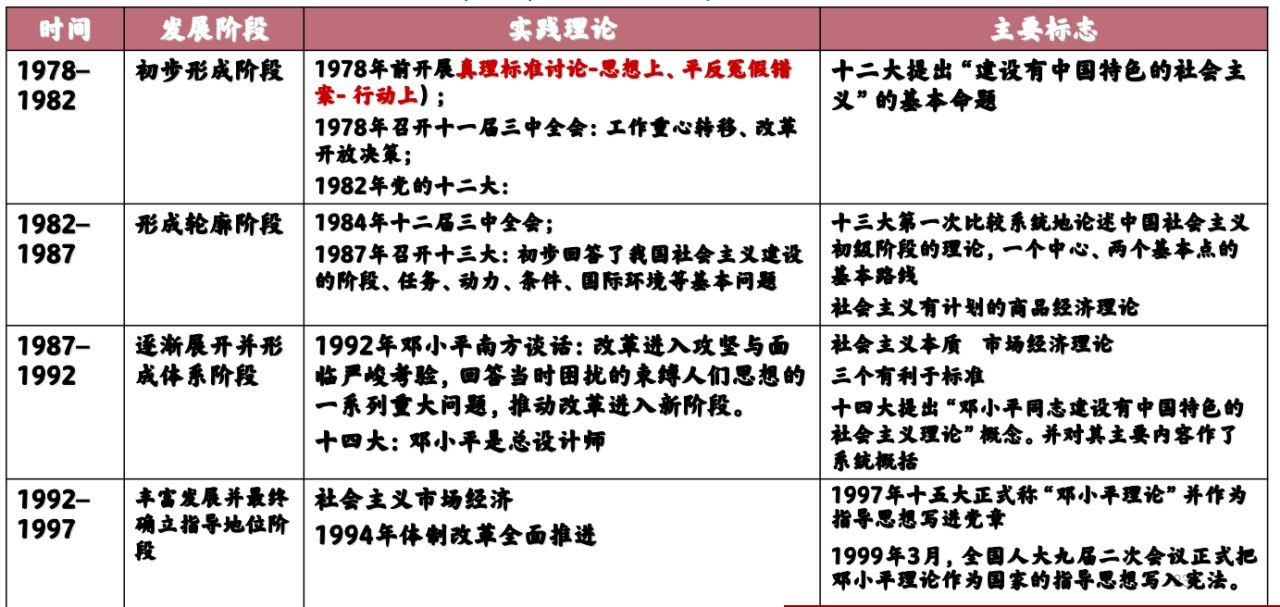
\includegraphics[width=0.95\linewidth]{fig-deng-lilun.png}\end{center}
\subsubsection{十一届三中全会在三方面的转折}
\begin{itemize}
  \item 思想路线：彻底否定“两个凡是”的方针，重新确立了\textbf{解放思想、实事求是}的思想路线
  \item 工作重心：停止使用“以阶级斗争为纲”的错误提法，确定把全党工作的着重点转移到\textbf{社会主义现代化建设}上来，作出实行改革开放的重大决策。
  \item 组织领导：实际上形成了\textbf{以邓小平为核心的党中央领导集体}
\end{itemize}
意义：十一届三中全会实现了党的历史上具有深远意义的伟大转折。
\subsubsection{党的十二大的意义}
第一次明确提出了“建设有中国特色的社会主义”的基本命题，回答了进入改革开放新时期后中国走什么样的道路这一人们最为关心的重大问题，成为指引新时期改革开放和社会主义现代化建设的伟大旗帜。从此，“\textbf{中国特色社会主义}”成为我们党的全部理论和实践创新的主题。
\subsubsection{党的十三大}
\begin{itemize}
  \item 党的十三大第一次比较系统地论述了我国社会主义初级阶段理论，明确概括和全面阐发了党的“\textbf{一个中心、两个基本点}”的基本路线。
  \item 意义：
\begin{itemize}
  \item 从马克思主义哲学、政治经济学和科学社会主义等方面，第一次对中国特色社会主义理论的主要内容作了系统概括。
  \item 这是我们党第一次对中国特色社会主义理论进行系统的概括，也标志着邓小平理论轮廓的形成。
\end{itemize}
\end{itemize}
\subsubsection{邓小平南巡讲话的重要论断}
\begin{itemize}
  \item 社会主义本质：\textbf{解放生产力，发展生产力，消灭剥削，达到共同富裕}
  \item “\textbf{三个有利于}”标准：是否有利于发展社会主义社会的生产力，是否有利于增强社会主义国家的综合国力，是否有利于提高人民的生活水平；
\begin{itemize}
  \item 社会主义可以搞市场经济；
  \item 革命是解放生产力，改革也是解放生产力；
  \item 不坚持社会主义，不改革开放，不发展经济，不改善人民生活，就没有出路；
  \item 改革开放的胆子要大一些，敢于试验，看准了的，就大胆地试，大胆地闯；
  \item 要提倡科学，靠科学才有希望；
\end{itemize}
  \item “两手抓，两手都要硬”：要坚持两手抓，一手抓改革开放，一手抓打击各种犯罪活动，这两手都要硬。
\end{itemize}
意义：南方谈话是邓小平理论的集大成之作，邓小平理论也逐步走向成熟。
\subsubsection{邓小平理论的最终形成与确立}
\begin{itemize}
  \item 1997年召开的\textbf{党的十五大正式}提出“邓小平理论”这一概念，深刻阐述了邓小平理论的历史地位和指导意义，进一步论述了邓小平对这一理论的创立作出的独创性贡献。
  \item \textbf{1999年}，宪法修正案正式将邓小平理论载入宪法
  \item 邓小平理论的地位和价值：第一次比较系统地初步回答了在中国这样的经济文化比较落后的国家如何建设社会主义、如何巩固和发展社会主义的一系列基本问题，用新的思想观点，继承和发展了马克思主义，开拓了马克思主义新境界，把对社会主义的认识提高到新的科学水平，是中国特色社会主义理论体系的开篇之作。
\end{itemize}
\subsection{中国特色社会主义理论体系的跨世纪发展丨“三个代表”重要思想}
\begin{itemize}
  \item “三个代表”重要思想的科学内涵和基本内容
\begin{itemize}
  \item “三个代表”重要思想是我们党坚持以马克思列宁主义、毛泽东思想、 邓小平理论和党的基本路线为指导
  \item 以我国改革开放和现代化建设的实际问题、以我们正在做的事情为中心
  \item 着眼于马克思主义理论的运用，着眼于对现实问题的思考，着眼于新的实践和新的发展
  \item 对党在现阶段以至今后相当长的历史时期中的基本纲领、基本任务的新概括
\end{itemize}
  \item “三个代表”重要思想的意义和地位
\begin{itemize}
  \item \textbf{加深了对什么是社会主义、怎样建设社会主义}和\textbf{建设什么样的党、怎样建设党}的认识，积累了治党治国新的宝贵经验。
  \item 反映了当代世界和中国的发展变化对党和国家工作的新要求，是加强和改进党的建设、推进我国社会主义自我完善和发展的强大理论武器，是中国共产党集体智慧的结晶，丰富和发展了中国特色社会主义理论体系
  \item 始终做到“三个代表”，是我们党的立党之本、执政之基、力量之源。
\end{itemize}
  \item 建设中国特色社会主义的十条基本经验
\begin{enumerate}
  \item 坚持以邓小平理论为指导，不断推进理论创新
  \item 坚持以经济建设为中心，用发展的办法解决前进中的问题
  \item 坚持改革开放，不断完善社会主义市场经济体制
  \item 坚持四项基本原则，发展社会主义民主政治
\end{enumerate}
\begin{itemize}
  \item 四项基本原则：必须坚持社会主义道路；必须坚持无产阶级专政；必须坚持党的领导；必须坚持马列主义、毛泽东思想。
\end{itemize}
\begin{enumerate}
  \item 坚持物质文明和精神文明两手抓，实行依法治国和以德治国相结合
  \item 坚持稳定压倒一切的方针，正确处理改革发展稳定的关系
  \item 坚持党对军队的绝对领导，走中国特色的精兵之路
  \item 坚持团结一切可以团结的力量，不断增强中华民族的凝聚力
  \item 坚持独立自主的和平外交政策，维护世界和平与促进共同发展
  \item 坚持加强和改善党的领导，全面推进党的建设新的危大工程
\end{enumerate}
\end{itemize}
\subsection{中国特色社会主义理论体系在新世纪新阶段的新发展丨科学发展观}
\begin{itemize}
  \item 科学发展观在抗击非典疫情和探索完善社会主义市场经济体制的过程中逐步形成。
  \item 2004年3月，胡锦涛在中央人口资源环境座谈会上发表重要讲话，深刻阐明了科学发展观提出的背景、意义，明确界定了“以人为本”“全面发展”“协调发展”“可持续发展”的深刻内涵和基本要求，并对如何树立和落实科学发 展观提出了明确的要求，标志着科学发展观的形成。
  \item 科学发展观的意义和地位：
\begin{itemize}
  \item 科学发展观总结了二十多 年来我国改革开放和现代化建设的成功经验，揭示了经济社会发展的客观规律，反映了我们党对发展问题的新认识
  \item 科学发展观对整个改革开放和 现代化建设都具有重要指导意义：只有贯彻落实好科学发展观，才能确保 全面建成小康社会、基本实现现代化
  \item 科学发展观是马克思主义同当代中国实际和时代特征相结合的产物， 是马克思主义关于发展的世界观和方法论的集中体现
  \item 对新形势下实现什么样的发展、怎样发展等重大问题作出了新的科学回答，把我们对中国特色社会主义规律的认识提高到新的水平
\end{itemize}
\end{itemize}
\subsection{中国特色社会主义理论体系在新时代的新篇章丨习近平新时代中国特色社会主义思想}
\begin{itemize}
  \item 党的十九大、十九届六中全会提出的“十个明确”“十四个坚持” “十三个方面成就”概括了习近平新时代中国特色社会主义思想的主要内容
  \item 习近平新时代中国特色社会主义思想的意义和地位：
\begin{itemize}
  \item \textbf{习近平新时代中国特色社会主义思想科学回答了新时代坚持和发展什么样的中国特色社会主义、怎样坚持和发展中国特色社会主义，建设什么样的社会主义现代化强国、怎样建设社会主义现代化强国，建设什么样的长期执政的马克思主义政党、怎样建设长期执政的马克思主义政党等重大 时代课题。}
  \item 习近平新时代中国特色社会主义思想是对马克思列宁主义、毛泽东思想、邓小平理论、“三个代表”重要思想、科学发展观的继承和发展，是当代中国马克思主义、21世纪马克思主义，是中华文化和中国精神的时代精华，是党和人民实践经验和集体智慧的结晶，是中国特色社会主义理 论体系的重要组成部分，是全党全国人民为实现中华民族伟大复兴而奋斗 的行动指南。
  \item 中国特色社会主义理论体系是中国共产党长期探索的伟大理论创造， 同马克思列宁主义、毛泽东思想一脉相承又与时俱进，是马克思主义中国 化时代化的重大理论成果；它以全新的视野进一步深化和丰富了对共产党 执政规律、社会主义建设规律、人类社会发展规律的认识，是内涵丰富、 思想深刻、系统完整的科学理论体系。
\end{itemize}
\end{itemize}
\chapter{邓小平理论}
\textbf{什么是社会主义、怎样建设社会主义}是邓小平理论要回答的首要的基本的理论问题。解放思想、实事求是是邓小平理论的精髓。邓小平理论在社会主义发展道路、发展阶段、根本任务、发展动力、 外部条件、政治保证、战略步骤、领导力量和依靠力量、祖国统一等重大 问题上，形成了一系列相互联系的基本观点，构成了科学的理论体系。邓小平理论是对马克思列宁主义、毛泽东思想在新的历史条件下的继承和发展，是中国特色社会主义理论体系的开篇之作，对改革开放和社会 主义现代化建设具有长远的指导意义。
\section{邓小平理论首要的基本的理论问题和精髓}
\subsection{社会主义本质论}
（来自课件）
\begin{itemize}
  \item 社会主义本质的内容：\textbf{解放生产力、发展生产力、消灭剥削、消除两极分化、最终达到共同富裕}
  \item 社会主义本质论的深入分析
\begin{itemize}
  \item 既包括了社会主义社会的生产力问题，又包括了以社会主义生产关系为基础的社会关系问题，是一个有机的整体
  \item 突出强调了“最终实现共同富裕”的目标，为我们既坚持公有制又完善和发展公有制指出了明确的方向
\end{itemize}
  \item 邓小平关于社会主义本质的概括的意义
\begin{itemize}
  \item 对于我们在坚持社会主义基本制度的基础上推进改革，具有重大的政治意义
  \item 对于我们指导改革沿着合乎社会主义本质要求的方向发展，具有重大的理论意义
  \item 对于我们建设中国特色的社会主义，具有重大的实践意义
\end{itemize}
\end{itemize}
\subsection{邓小平理论首要的基本的理论问题}
\begin{itemize}
  \item 搞清楚“什么是社会主义，怎样建设社会主义”，关键是要\textbf{在坚持社会主义基本制度的基础上进一步认清社会主义的本质}。
  \item 社会主义最大的优越性就是\textbf{共同富裕}，这体现了社会主义的本质。
  \item 1992年初，邓小平在南方谈话中对社会主义本质作出了总结性的理论概括，他指出：“社会主义的本质，是解放生产力，发展生产力，消灭 剥削，消除两极分化，最终达到共同富裕。”     
\begin{itemize}
  \item 这一科学概括，既坚持了科学社会主义的基本原则，又赋予其鲜明的时代特色，是探索中国特色社会主义取得的重大理论成果之一，是对马克思主义的重大发展。
  \item 首先，它突出地强调解放和发展生产力在社会主义社会发展中的重要地位，纠正了过去关于发展生产力的一些错误观念，反映了中国社会主义整个历史阶段尤其是初级阶段特别需要注重生产力发展的迫切要求，并明确了社会主义基本制度建立后还要通过改革进一步解放生产力。
  \item 其次，它突出地强调“消灭剥削，消除两极分化，最终达到共同富裕”，从生产关系和发展目标角度认识和把握社会主义本质。
\end{itemize}
  \item 邓小平关于社会主义本质的概括，反映了人民的利益和时代的要求，廓清了不合乎时代进步和社会发展规律的模糊观念，摆脱了长期以来拘泥于具体模式而忽略社会主义本质的错误倾向，把对社会主义的认识提高到 新的科学水平。这对于我们在坚持社会主义基本制度的基础上推进改革， 指导改革沿着合乎社会主义本质要求的方向发展，对于建设中国特色社会 主义，具有重大的\textbf{政治意义、理论意义和实践意义}。
\end{itemize}
\subsection{邓小平理论的精髓}
\subsubsection{邓小平理论的精髓和活的灵魂}
（来自课件）
\begin{itemize}
  \item 解放思想 、实事求是的思想路线是邓小平理论的精髓和活的灵魂**
\begin{itemize}
  \item 第一，坚持解放思想、实事求是，有力推动和保证了拨乱反正的进行。
  \item 第二，坚持解放思想、实事求是，破除了僵化的社会主义模式观念，坚持走自己的路。
  \item 第三，坚持解放思想、实事求是，一切从社会主义初级阶段的实际出发。
  \item 第四，坚持解放思想、实事求是，坚持以“三个有利于”作为检验一切工作是非得失的根本标准，破除了在改革开放进程中离开发展生产力抽象谈论姓“社”姓“资”的思维定势，把我 国的改革开放和现代化建设推进到一个新的阶段。
\end{itemize}
  \item 意义和价值
\begin{itemize}
  \item 推动和保证了改革开放的进行
  \item 体现了辩证唯物主义和历史唯物主义的世界观方法论
  \item 体现了革命胆略和科学精神的统一
\end{itemize}
\end{itemize}
\section{邓小平理论的主要内容}
\begin{itemize}
  \item 社会主义初级阶段理论
  \item 党的基本路线
  \item 社会主义根本任务理论
  \item “三步走”战略
  \item 改革开放理论
  \item 社会主义市场经济理论
  \item “两手抓，两手都要硬”
  \item “一国两制”与祖国统一
  \item 中国特色社会主义外交和国际战略
  \item 党的建设理论
\end{itemize}
\subsection{社会主义初级阶段理论和党的基本路线}
\subsubsection{社会主义初级阶段理论}
\begin{itemize}
  \item 社会主义初级阶段的含义：我国在生产力落后、商品经济不发达条件下建设社会主义必然要经历的特定阶段，即从我国进入社会主义到基本实现社会主义现代化的整个历史阶段。
  \item 正确认识党和人民事业所处的历史方位和发展阶段，是我们党明确阶段性中心任务、制定路线方针政策的根本依据，也是我们党领导革命、建设、改革不断取得胜利的重要经验。
  \item 如何科学认识和判断所处历史方位和发展阶段，是我国社会主义建设必须解决的重大理论问题和实践问题。
  \item 党的十三大系统地阐述了\textbf{社会主义初级阶段的科学内涵}。首先，阐明了 社会主义初级阶段这个论断包括两层含义：
\begin{itemize}
  \item 第一，我国社会已经是社会主义社会。我们必须坚持而不能离开社会主义；
  \item 第二，我国的社会主义社会还处在初级阶段。我们必须从这个实际出发，而不能超越这个阶段；
  \item 第一层含义阐明了初级阶段的社会性质，第二层含义阐明了我国社会主义社会的发展程度，两层含义不可分割，必须全面把握。只有把社会主义社会的性质同它的发展程度有机地统一起来，才能够深刻地理解和把握我国的基本国情。
\end{itemize}
  \item 强调了社会主义初级阶段的长期性。
  \item 阐述了社会主义初级阶段的基本特征：既不同于社会主义经济基础尚未奠定的过渡时期，又不同于已经实现社会主义现代化的阶段。
  \item 社会主义初级阶段理论基于对中国国情的准确把握，揭示了当代中国的\textbf{历史方位}，是对马克思主义关于社会主义发展阶段理论的重大发展和重大突破，为建设中国特色社会主义提供了\textbf{总依据}。
\end{itemize}
\subsubsection{党在社会主义初级阶段的基本路线}
\begin{itemize}
  \item 党的十三大提出了党在社会主义初级阶段的基本路线：“\textbf{领导和团结全国各族人民，以经济建设为中心，坚持四项基本原则，坚持改革开放，自力更生，艰苦创业，为把我国建设成为富强、民主、文明的社会主义现代化国家而奋斗}。”
  \item 党的基本路线高度概括了党在社会主义初级阶段的\textbf{奋斗目标、领导力量和依靠力量、基本途径和根本保证}以及实现这一目标的\textbf{基本方针}。
\begin{itemize}
  \item 首先，\textbf{建设“富强、民主、文明的社会主义现代化国家”是党在社会主义初级阶段的奋斗目标}。三者在现实中表现为经济建设、政治建设、文化建设的统一。
  \item 其次，\textbf{“以经济建设为中心，坚持四项基本原则，坚持改革开放”是实现奋斗目标的基本途径}（“一个中心，两个基本点”）。
\begin{itemize}
  \item “以经济建设为中心”回答了社会主义的根本任务问题
  \item “坚持四项基本原则”回答了解放和发展生产力的政治保证问题
  \item “坚持改革开放”回答了社会主义的发展动力和外部条件问题。
  \item 以经济建设为中心是党在改革开放和社会主义现代化建设新时期实现的最根本的拨乱反正。四项基本原则是立国之本，是我们党和国家生存发展的政治基石；改革开放是强国之路，是我们党和国家发展进步的活力源泉。它们是一个整体，集中体现了我国社会主义现代化建设的战略布局，揭示了中国特色社会主义的客观规律和发展道路。
\end{itemize}
  \item 再次，\textbf{“领导和团结各族人民”是实现奋斗目标的领导力量和依靠力量}。中国共产党是中国特色社会主义事业的领导核心，中国特色社会主义事业要紧紧依靠全国各族人民，有了这两者的结合，社会主义现代化事业就必定能够胜利。
  \item 最后，\textbf{“自力更生，艰苦创业”是实现奋斗目标的根本立足点}。把“自力更生，艰苦创业”方针概括到党的基本路线之中，不仅是改变我国不发达现状的需要，也体现了社会主义的奋斗精神。
\end{itemize}
\end{itemize}
\subsection{社会主义根本任务和发展战略理论}
\subsubsection{社会主义根本任务的理论}
\begin{itemize}
  \item 生产力是社会发展的最根本的决定性因素，马克思主义始终高度重视 生产力的发展。党的十一届三中全会以后，我们党把工作重点转移到经济建设上来，强调社会主义的根本任务是发展生产力。
  \item 邓小平还强调，社会主义制度优越性的根本表现，就是能够允许社会生产力以旧社会所没有的速度迅速发展，使人民不断增长的物质文化生活需要能够逐步得到满足；
  \item 中国解决所有问题的关键是要靠自己的发展。
  \item 邓小平关于“科学技术是第一生产力”的重大论断，继承发展了马克思主义关于科学技术是生产力的论点，反映了...（灵活发挥）
\end{itemize}
\subsubsection{分三步走基本实现现代化的发展战略}
\begin{itemize}
  \item “三步走”的发展战略内容：
\begin{itemize}
  \item 第一步：到1990年，实现国民生产总值比1980年翻一番，解决人民的\textbf{温饱}问题
  \item 第二步：到20世纪末，使国民生产总值再增长一倍，人民生活达到\textbf{小康}水平
  \item 第三步：到21世纪中叶，人均国民生产总值达到中等发达国家水平，人民生活比较富裕，\textbf{基本实现现代化}。然后，在这个基础上继续前进。
\end{itemize}
  \item “三步走”的发展战略，把我国社会主义现代化建设的目标具体化为切实可行的步骤，为基本实现现代化明确了发展方向，展现了美好的前景，成为全国人民团结奋斗的行动纲领。
  \item 1982年9月，邓小平提出三个战略重点：一是农业，二是能源和交通，三是教育和科学。
  \item 为了更好地实现现代化发展战略，邓小平提出了 “台阶式”发展的思想。
  \item 为了更好地实现“三步走”的发展战略，邓小平还提出允许和鼓励一部分地区、一部分人先富起来逐步实现共同富裕的思想。
\end{itemize}
\subsection{社会主义改革开放和社会主义市场经济理论}
\subsubsection{社会主义改革开放理论}
\begin{itemize}
  \item 党的\textbf{十一届三中全会}作出把党和国家工作中心转移到\textbf{经济建设}上来、 实行改革开放的历史性决策
  \item 改革是社会主义社会发展的直接动力。\textbf{社会主义社会的基本矛盾仍然是生产关系和生产力、上层建筑和经济基础之间的矛盾}，正是这些矛盾运动推动了社会主义社会的发展。
\begin{itemize}
  \item 改革是一场深刻的社会变革，是中国的第二次革命，是实现中国现代化的必由之路。改革不是原有经济体制的细枝末节的修补，它的实质和目标是要从根本上改变束缚我国生产力发展的经济体制，建立充满生机和活力的社会主义新经济体制，同时相应地改革政治体制和其他方面的体制，以实现中国的社会主义现代化。（仅作了解）
\end{itemize}
  \item 改革是一项崭新的事业，是一个大试验。主要看是否有利于发展社会主义社会的生产力，是否有利于增强社会主义 国家的综合国力，是否有利于提高人民生活水平，即\textbf{“三个有利于”标准}。“三个有利于”标准是内在统一的，发展社会主义社会的生产力是首要的也是最根本的一条，增强社会主义国家的综合国力和提高人民生活 平是以生产力发展为前提，也是发展生产力的目的。
  \item 开放也是改革，对外开放是建设中国特色社会主义的一项基本国策，和改革一起成为新时期最鲜明的特征。
\begin{itemize}
  \item 实行对外开放是对中国经济发展停滞落后历史教训深刻总结的结果。
  \item 对外开放是对世界所有国家的开放，包括对发达国家的开放，也包括对发展中国家的开放；不仅是经济领域的开放，还包括科技、教育、文化 等领域的开放。
\end{itemize}
  \item 实践证明，\textbf{改革开放是当代中国的鲜明标志和活力源泉，是决定中国命运的关键一招，也是实现中华民族伟大复兴的关键一招}。改革开放只有进行时，没有完成时，必须毫不动摇地坚持。
\end{itemize}
\subsubsection{社会主义市场经济理论}
\begin{itemize}
  \item “计划多一点还是市场多一点，不是社会主义与资本主义的本质区别。计划经济不等于社会主义，资本主义也有计划；市场经济不等于资本主义，社会主义也有市场。计划和 市场都是经济手段。”这一精辟论述，从理论上突破了计划经济和市场经济是制度属性的观念，从根本上解除了把计划经济和市场经济看做属于社会基本制度范畴的思想束缚，标志着\textbf{邓小平的社会主义市场经济理论的形成}。这也为党的十四大明确把建立社会主义市场经济体制作为我国经济体制改革的目标奠定了理论基础。
  \item 邓小平的社会主义市场经济理论具有丰富的内涵
\begin{itemize}
  \item 一是\textbf{计划经济和市场经济不是划分社会制度的标志}；
  \item 二是\textbf{计划和市场都是经济手段}，对经济活动的调节各有优劣，社会主义实行市场经济是要把两者优势结合起来；
  \item 三是\textbf{市场经济作为资源配置手段本身不具有制度属性}，可以和不同的社会制度结合，从而表现出不同的性质。坚持社会主义制度与市场经济的结合，是社会主义市场经济的特色所在、优势所在。
\end{itemize}
  \item 邓小平的社会主义市场经济理论，实现了马克思主义政治经济学的重大创新，是中国特色社会主义政治经济学的重要组成部分，为社会主义市场经济体制改革目标的确立和中国特色社会主义经济建设提供了指南。
\end{itemize}
\subsection{“两手抓，两手都要硬”}
\begin{itemize}
  \item \textbf{社会主义精神文明是社会主义社会的重要特征}，社会主义发展应实现\textbf{物质}文明与\textbf{精神}文明的共同进步。
  \item 在邓小平社会主义精神文明建设思想中，一手抓物质文明，一手抓精神文明，“两手抓，两手都要硬”具有鲜明的特色。
\begin{itemize}
  \item 首先，强调我们要建设的社会主义国家，不但要有高度的物质文明，而且要有高度的精神文明；
  \item 其次，强调物质文明建设和 精神文明建设相辅相成、相互促进；
  \item 最后，强调精神文明重在建设。精神文 明具有自身内在的发展规律，有着历史的继承性，它与物质文明有着不平衡性、不同步性的关系，精神文明重在建设，所以要“抓”精神文明建 设，不但要“抓”并且要“硬”。
\end{itemize}
  \item 提出\textbf{以经济建设为中心，坚定不移地进行经济体制改革，坚定不移地进行政治体制改革，坚定不移地加强精神文明建设}，并且使这几个 方面互相配合、互相促进，初步形成了我国社会主义现代化建设“三位一体”的总体布局。
  \item “一手抓建设，一手抓法制”。发展社 会主义民主，健全社会主义法制，是党的十一届三中全会以来我们党坚定 不移的基本方针。
  \item “一手抓改革开放，一手抓惩治腐败”。
  \item 邓小平的一系列“两手抓”，坚持了辩证法的全面性，坚持了两点论 和重点论的统一，有利于克服实际工作中存在的“一手硬、一手软”的问 题，为我们党的领导方法和工作方法充实了新的内容。
\end{itemize}
\subsection{“一国两制”与祖国统一}
实现祖国的完全统一，是国家繁荣富强和民族伟大复兴的基础，是海内外中华儿女的共同心愿，是中华民族的根本利益所在，是中国共产党和中国人民不可动摇的坚强意志。
\begin{itemize}
  \item “一国两制”包含着丰富的科学内涵。其基本内容有
\begin{itemize}
  \item \textbf{坚持一个中国，这是“和平统一、 一国两制”的核心，是发展两岸关系和实现和平统一的基础}；
  \item 两制并存， 在祖国统一的前提下，国家的主体部分实行社会主义制度，同时在香港澳门、台湾保持原有的社会制度和生活方式长期不变；
  \item 高度自治，祖国完全统一后，香港、澳门、台湾作为中央政府全面管辖下的特别行政区，享 有不同于中国其他省、市、自治区的高度自治权，台湾、香港、澳门同胞 各种合法权益将得到切实尊重和维护；
  \item \textbf{尽最大努力争取和平统一，但不承诺放弃使用武力}；
  \item 解决台湾问题，实现祖国完全统一，寄希望于台湾人民。
\end{itemize}
  \item “一国两制”构想是邓小平运用辩证唯物主义和历史唯物主义，坚持实事求是，把和平共处原则用于解决一个国家的统一问题，既体现了坚 持祖国统一、维护国家主权的原则性，又体现了照顾历史实际和现实可能的灵活性，是对马克思主义国家学说的创造性发展。
\end{itemize}
\subsection{中国特色社会主义外交和国际战略}
\begin{itemize}
  \item 1987年，党的十三大确认了\textbf{和平与发展}是当今世界的两大主题这一深刻论断。
  \item 邓小平对时代主题的判断基本点（仅作了解）
\begin{itemize}
  \item 第一，世界大战在一个相当 长的时期内可以避免，我们有可能争取较长时期的和平环境；
  \item 第二，从经济角度来说，和平与发展是当今世界两大带有全球性的战略问题，是东西方之间、发达国家与发展中国家之间矛盾全局的集中体现；
  \item 第三，和平与发展是相辅相成的，世界和平是促进各国共同发展的前提条件，各国的共 同发展则是保持世界和平的重要基础；
  \item 第四，和平与发展成为时代主题，并不意味着这两个问题已经解决。要清醒地看到，当今世界和平与发展这两大问题一个都没有得到解决，还需要各国人民长期不懈地共同努力。
\end{itemize}
  \item \textbf{明确维护我国的独立和主权，促进世界的和平与发展，是中国外交政策的基本目标}。
  \item \textbf{坚持在和平共处五项原则的基础上，建立和平、稳定、公正、合理的国际新秩序}。
  \item 坚持以\textbf{独立自主、完全平等、互相尊重、互不干涉内部事务原则}处理 同各国共产党和其他政党的关系。党与党之间的关系是平等的关系，任何 国家的事情只能由那个国家的党和人民去判断。
  \item 邓小平外交思想的概述（仅作了解）：关于外交工作，邓小平强调要反对霸权主义，维护世界和平，为我国 社会主义现代化建设争取一个较长时期的国际和平环境；坚持在和平共处 五项原则基础上发展同所有国家的友好合作关系；高度重视第三世界国家 的战略地位和作用，强调加强同它们的团结与合作；主张积极推动建立和 平稳定、公正合理的国际政治经济新秩序；强调坚定不移地实行对外开放 政策；确定了冷静观察、稳住阵脚、沉着应付、韬光养晦、有所作为、善于守拙、决不当头的方针；确立党际关系“四项原则”，开创党的对外工 作新局面；强调中国是维护世界和平与稳定的力量，要对人类进步事业作出更大的贡献。
\end{itemize}
\subsection{党的建设理论}
\begin{itemize}
  \item \textbf{建设中国特色社会主义，关键在于坚持、加强和改善党的领导}。
  \item 加强党的建设，是我们党领导人民取得革命和建设胜利的法宝。 
  \item 重视马克思主义理论学习是加强党的建设，从而增强我们工作中的原 则性、系统性、预见性和创造性的必修课。
  \item \textbf{加强组织建设是党的建设的重要环节}。党的基层组织是党的全部工作和战斗力的基础。坚持和健全民主集中制、加强和改进党的基层组织建 设、培养和选拔德才兼备的领导干部是组织建设的重要问题。民主集中制是党的根本组织制度和领导制度，是最便利、最合理的制度。
  \item 加强领导班子建设，培养和选拔德才兼备的各级领导干部，是加强 党的建设，保证党的路线的连续性和国家长治久安的根本大计。
  \item 加强党的建设必须打好党风建设这场硬仗。\textbf{执政党的党风关系党的生死存亡}。
  \item 在社会主义的依靠力量问题上，强调\textbf{人民群众是我们党的力量源泉和胜利之本}。
  \item 在人民军队建设问题上，强调党领导的人民军队是社会主义祖国的保卫者和建设社会主义的重要力量，要坚持\textbf{党对军队的绝对领导}。
\end{itemize}
\section{邓小平理论的历史地位}
\subsection{马克思列宁主义、毛泽东思想的继承和发展}
\begin{itemize}
  \item 邓小平理论是马克思列宁主义基本原理同当代中国实际和时代特征相 结合的产物，是对马克思列宁主义、毛泽东思想的继承和发展，是全党全 国人民集体智慧的结晶。
  \item 邓小平是我国改革开放和社会主义现代化建设的总设计师，对邓小平理论的创立作出了历史性的重大贡献。
  \item 邓小平理论坚持解放思想、实事求是，在新的实践基础上既继承前人又突破陈规，开拓了马克思主义的新境界。
  \item \textbf{解放思想、实事求是}是邓小平理论的精髓。
  \item 邓小平理论坚持马克思列宁主义、毛泽东思想的基本原理， 坚持辩证唯物主义和历史唯物主义的立场观点方法，坚持马克思主义的思 想路线，围绕\textbf{什么是社会主义、怎样建设社会主义}的问题，系统回答了在中国这样经济文化比较落后的东方大国建设、巩固和发展社会主义的 一系列基本问题，用一系列独创性的思想、观点，继承、丰富和发展了马克思列宁主义、毛泽东思想。
\end{itemize}
\subsection{中国特色社会主义理论体系的开篇之作}
\begin{itemize}
  \item 邓小平深刻总结我国社会主义建设正反两方面经验，借鉴世界社会主义历史经验，作出把党和国家的工作中心 转移到经济建设上来、实行改革开放的历史性决策，科学回答了建设中国 特色社会主义的一系列基本问题，成功开创了中国特色社会主义。
  \item 邓小平 开创性地提出了社会主义本质、社会主义初级阶段、党的基本路线、改 革开放、“一国两制”等一系列具有浓厚中国特色的新概念新范畴，建构 了中国特色社会主义理论的基本框架。
  \item 邓小平理论第一次比较系统地初步回答了建设中国特色社会主义的一 系列基本问题，包括社会主义初级阶段理论，党在社会主义初级阶段的基 本路线，社会主义根本任务和发展战略，社会主义改革开放理论，社会主 义市场经济理论，“两手抓，两手都要硬”，“一国两制”和实现祖国统一， 中国特色社会主义外交和国际战略，党的建设理论等，形成了一个比较完备的科学体系。
\end{itemize}
\subsection{改革开放和社会主义现代化建设的科学指南}
\begin{itemize}
  \item 邓小平理论指导了改革开放的伟大实践
\begin{itemize}
  \item 邓小平强调必须坚持以经济建设为中心，坚持四项基本原则，坚持改革开放，领导党制定了党在社会主义初级阶段的基本路线；
  \item 指导我们党正确认识我国所处的发展阶段 和根本任务，制定了现代化建设“三步走”发展战略；突出强调“改革是中国的第二次革命”，领导我们党有步骤地展开各方面体制改革，勇敢打开对外开放的大门；
  \item 反复强调“两手抓，两手都要硬”，必须抓好社会主义精神文明建设和民主法制建设，实现社会全面进步；
  \item 创造性提出“一国 两制”科学构想，指导我们实现香港、澳门平稳过渡和顺利回归，推动海 峡两岸关系打开新局面；
  \item 明确提出和平与发展是当代世界的两大主题，领导我们党及时调整各方面政策，为改革开放和社会主义现代化建设创造了难得历史机遇和良好外部环境；
  \item 强调加强党的领导必须改善党的领导，必须聚精会神抓党的建设，使党的建设充满新的生机活力。
\end{itemize}
  \item 邓小平理论是邓小平留给我们的最重要的思想遗产。邓小平理论是中国共产党和中国人民宝贵的精神财 富，是改革开放和社会主义现代化建设的科学指南，是党和国家必须长期坚持的指导思想。
\end{itemize}
\chapter{“三个代表”重要思想}
\textbf{“三个代表”重要思想的形成条件}
（根据往年知识点整理额外补充）
\begin{itemize}
  \item “三个代表”重要思想是在对冷战结束后国际局势科学判断的基础上形成的
  \item “三个代表”重要思想是在科学判断党的历史方位和总结历史经验的基础上提出的
  \item “三个代表”重要思想是在建设中国特色社会主义伟大实践基础上形成的
\end{itemize}
\section{“三个代表”重要思想的核心观点}
“三个代表”重要思想的三条内容是统一的整体，相互联系、相互促进。发展先进生产力，是发展先进文化、实现最广大人民根本利益的基础条件。人民群众是先进生产力和先进文化的创造主体，也是实现自身利益的根本力量。不断发展先进生产力和先进文化，归根到底都是为了满足人民群众日益增长的物质文化生活需要，不断实现最广大人民的根本利益。
\subsection{始终代表中国先进生产力的发展要求}
始终代表中国先进生产力的发展要求，就是党的理论、路线、纲领、方针、政策和各项工作，必须努力\textbf{符合生产力发展的规律，体现不断推动社会生产力的解放和发展的要求}，尤其要体现推动先进生产力发展的要 求，通过发展生产力不断提高人民群众的生活水平。
\begin{itemize}
  \item \textbf{社会主义的根本任务是发展社会生产力}，马克思主义执政党必须高度重视解放和发展生产力。
\begin{itemize}
  \item 我们党建立时就是以中国先进生产力的代表走上历史舞台的。
  \item 社会主义现代化必须建立在发达生产力的基础之上。
  \item 广大工人、农民和知识分子始终是推动我国先进生产力发展和社会全面进步的根本力量。
  \item 人是生产力中最活跃的因素。开发人力资源，加强人力资源能力建设，是关系我国发展的重大问题，必须树立人才资源是第一资源的思想， 紧紧抓住培养人才、吸引人才、用好人才三个环节，大力实施人才战略， 加强人才队伍建设。
\end{itemize}
  \item “科学技术是第一生产力，是先进生产力的集中体现和主要标志”。
  \item 先进生产力的发展是同生产关系、上层建筑的不断完善密切联系在一起的。
\end{itemize}
\subsection{始终代表中国先进文化的前进方向}
始终代表中国先进文化的前进方向，就是党的理论、路线、纲领、方针、政策和各项工作，必须努力体现\textbf{发展面向现代化、面向世界、面向未来的，民族的科学的大众的社会主义文化的要求}，促进全民族思想道德素质和科学文化素质的不断提高，为我国经济发展和社会进步提供精神动力和智力支持。
\begin{itemize}
  \item 发展先进文化，是实现社会主义现代化的战略任务。
  \item 发展先进文化，就是发展中国特色社会主义的文化，就是建设社会主义精神文明。
  \item 发展先进文化，就是发展面向现代化、面向世界、面向未来的，民族的科学的大众的社会主义文化。
  \item 发展先进文化，要把弘扬主旋律和提倡多样化统一起来，支持健康有益文化，努力改造落后文化，坚决抵制腐朽文化。
\begin{itemize}
  \item 加强社会主义思想道德建设，是发展先进文化的重要内容和中心环节。
  \item 做好思想政治工作是发展先进文化的重要任务。
  \item 教育是发展先进文化、建设物质文明和精神文明建设的基础工程。
  \item 繁荣发展哲学社会科学，是发展先进文化、建设社会主义精神文明的重要组成部分。
\end{itemize}
  \item 发展先进文化，需要充分发挥新闻媒体的作用。
  \item 发展先进文化，需要重视社会主义文艺事业的繁荣发展。
  \item 发展先进文化，必须大力推进文化体制改革。
\end{itemize}
\subsection{始终代表中国最广大人民的根本利益}
始终代表中国最广大人民的根本利益，就是党的理论、路线、纲领、方针、政策和各项工作，必须\textbf{坚持把人民的根本利益作为出发点和归宿， 充分发挥人民群众的积极性主动性创造性}，在社会不断发展进步的基础上，使人民群众不断获得切实的经济、政治、文化利益。
\begin{itemize}
  \item 人民是我们国家的主人，是决定我国前途和命运的根本力量，是历史的真正创造者。
\begin{itemize}
  \item 我们党来自人民，植根于人民，服务于人民。
  \item 我们党始终坚持人民的利益高于一切。
\end{itemize}
  \item 在建设中国特色社会主义的进程中，全国人民的根本利益是一致的， 各种具体的利益关系和内部矛盾可以在这个基础上进行调节。
\begin{itemize}
  \item 关心群众、代表群众利益，必须十分具体地落实到解决群众生产和生活的实际问题上。
\end{itemize}
  \item “人民，只有人民，才是我们工作价值的最高裁决者。”江泽民强调。
\end{itemize}
\section{“三个代表”重要思想的主要内容}
\subsection{发展是党执政兴国的第一要务}
党要承担起推动中国社会进步的历史责任，必须始终紧紧抓住发展这个执政兴国的第一要务，把坚持党的先进性和发挥社会主义制度的优越性，落实到发展先进生产力、发展先进文化、实现最广大人民的根本利益上来，推动社会全面进步，促进人的全面发展。
\begin{itemize}
  \item 中国特色社会主义是靠发展来不断巩固和推进的。
\begin{itemize}
  \item 发展是国际竞争中赢得主动的需要。
  \item 用发展的办法解决前进中的问题，是改革开放以来我们的一条重要经验。
  \item 发展是硬道理，中国解决所有问题的关键在于依靠自己的发展。
  \item 发展要善于抓住机遇，珍惜机遇，用好机遇。
\end{itemize}
  \item 发展是社会主义物质文明、政治文明和精神文明的协调发展。
\begin{itemize}
  \item 发展包括促进人的全面发展。
\end{itemize}
  \item 要正确认识和处理改革、发展、稳定的关系。
  \item 发展必须毫不动摇地坚持党在社会主义初级阶段的基本路线。
\end{itemize}
\subsection{建立社会主义市场经济体制}
在社会主义条件下发展市场经济，是改革开放新的历史性突破，打开了我国经济、政治和文化发展的崭新局面，是前无古人的伟大创举，是中国共产党人对马克思主义发展作出的历史性贡献，具有特殊重要的意义。
\begin{itemize}
  \item 经济体制问题是改革开放面临的重要问题。
  \item 建立社会主义市场经济体制，必须坚持和完善公有制为主体、多种所有制经济共同发展的社会主义基本经济制度。
\begin{itemize}
  \item 按照社会主义市场经济的要求，进一步探索公有制特别是国有制的多种有效实现形式。
  \item 发挥市场机制的作用和国家宏观调控，是社会主义市场经济体制的本质要求。
\end{itemize}
  \item 完善适应社会主义市场经济体制的分配关系。
  \item 建立和完善社会保障体系，是建立社会主义市场经济体制的重要内容。
\end{itemize}
\subsection{全面建设小康社会}
\begin{itemize}
  \item 全面建设小康社会的奋斗目标，是立足于我国的基本国情提出的。
  \item 全面建设小康社会，是实现现代化建设第三步战略目标必经的承上启下的发展阶段，也是完善社会主义市场经济体制和扩大对外开放的关键阶段。
\end{itemize}
\subsection{建设社会主义政治文明}
\textbf{建设社会主义政治文明与物质文明、精神文明一起确立为社会主义现代化全面发展的三大基本目标}，从而使中国特色社会主义的理论和实践进一步走向成熟和完善。建设社会主义政治文明，是我国改革开放和社会主义现代化建设发展的必然要求，是我们党领导人民坚持和发展人民民主长期实践的必然结论，进一步深化了我们党对中国特色社会主义事业的规律性认识。
\begin{itemize}
  \item 建设社会主义政治文明，发展社会主义民主政治，是社会主义现代化建设的重要目标。
\begin{itemize}
  \item 建设社会主义政治文明涉及政治思想、政治制度、行政管理、法制建设等方面，是一个系统工程。
\end{itemize}
  \item 建设社会主义政治文明，必须发展社会主义民主。
  \item 建设社会主义政治文明，必须坚持和完善中国特色社会主义政治制度。
  \item 建设社会主义政治文明，必须坚持依法治国，建设社会主义法治国家。
  \item 建设社会主义政治文明，必须进行政治体制改革。
  \item 建设社会主义政治文明，必须推进决策的科学化民主化。
  \item 建设社会主义政治文明，必须尊重和保障人权。
\end{itemize}
\subsection{实施"引进来”和"走岀去”相结合的对外开放战略}
对外开放是一项长期的基本国策。进入20世纪90年代，适应经济全球化趋势的发展和加入世界贸易组织的新形势，我国以更加积极的姿态走向世界，坚持“引进来”和“走出去”相结合，全面提高对外开放水平，在更大范围、更广领域和更高层次上参与国际经济技术合作和竞争，充分利用国际国内两个市场、两种资源，以开放促改革促发展。
\begin{itemize}
  \item 加入世界贸易组织，是以江泽民同志为主要代表的中国共产党人面对经济全球化趋势加快，从我国经济发展和改革开放的需要出发，作出的重大战略决策，标志着我国对外开放进入了一个新的阶段。
  \item 办好经济特区是继续推进我国改革开放和现代化建设的重大举措。
  \item “走出去”是对外开放新阶段的重大战略举措。
  \item 中国的发展和进步，离不开世界各国的文明成果——不管是哪种社会制度下创造的文明成果，只要是进步的优秀的东西，都应积极学习和运用。
  \item 在对外开放的过程中，始终耍注意维护国家的主权和经济社会安全。
\end{itemize}
\subsection{推进党的建设新的伟大工程}
\begin{itemize}
  \item 高度重视和不断加强自身建设，是我们党从小到大、由弱到强，从挫折中奋起、在战胜困难中不断成熟的一大法宝。
  \item 坚持中国共产党的领导，就是要坚持党在建设中国特色社会主义事业中的领导核心地位。
  \item 坚持中国共产党的领导，核心是坚持党的先进性。
  \item 推进党的建设新的伟大工程，重点是加强党的执政能力建设。
  \item 坚持用马克思主义武装全党。
  \item 民主集中制是我们党一贯坚持的根本组织制度和领导制度。
  \item 坚持党要管党、从严治党的方针。
\end{itemize}
\section{“三个代表”重要思想的历史地位}
\subsection{中国特色社会主义理论体系的丰富发展}
\begin{itemize}
  \item “三个代表”重要思想，坚持解放思想、实事求是、与时俱进，紧密结合时代发展的新形势，进一步把理论和实践、继承和发展结合起来，坚持以我国改革开放和现代化建设的实际问题、以我们正在做的事情为中心，着眼于马克思主义理论的运用，着眼于对实际问题的理论思考，着眼于新的实践和新的发展，回应我国广大人民群众的新要求，创造性地运用了马克思列宁主义、毛泽东思想特别是邓小平理论，形成了富有独创性的新的理论成果。“三个代表”重要思想，深化了我们对新的时代条件下推 进中国特色社会主义事业、加强党的建设的规律的认识，以新的思想、观点、论断，继承、丰富和发展了马克思列宁主义、毛泽东思想、邓小平理论，实现了党在指导思想上的又一次与时俱进。
  \item “三个代表”重要思想坚持把人民的根本利益作为岀发点和归宿。
  \item “三个代表”重要思想强调要努力促进人的全面发展。
  \item “三个代表”重要思想，把党的建设同世界的发展趋势，同我国社会主义的自我完善和发展，同实现中国特色社会主义的宏伟目标和各项任务联系起来。
\end{itemize}
\subsection{加强和改进党的建设、推进中国特色社会主义事业的强大理论武器}
\begin{itemize}
  \item “三个代表”重要思想在邓小平理论的基础上，进一步回答了\textbf{什么是社会主义、怎样建设社会主义的问题，创造性地回答了建设什么样的党、怎样建设党的问题，进一步深化了对中国特色社会主义的认识}。 “三个代表”重要思想反映了当代世界和中国的发展变化对党和国家工作的新要求，是加强和改进党的建设、推进我国社会主义自我完善和发展的强大理论武器，是党和国家必须长期坚持的指导思想，是党和人民的宝贵精神财富。
\end{itemize}
\chapter{科学发展观}
\textbf{科学发展观的形成条件}
（根据往年知识点整理额外补充）
\begin{itemize}
  \item 科学发展观是在深刻把握我国基本国情和新的阶段性特征的基础上形成和发展的(经济社会发展呈现一系列新的阶段性特征)
  \item 科学发展观是在深入总结改革开放以来特别是党的十六大以来实践经验的基础上形成和发展的
  \item 科学发展观是在深刻分析国际形势、顺应世界发展趋势、借鉴国外发展经验的基础上形成和发展的
\end{itemize}
\section{科学发展观的科学内涵}
\subsection{推动经济社会发展是科学发展观的第一要义}
发展是人类文明进步的基础，也是马克思主义最基本的范畴之一。我们党执政，首要任务就是带领人民推动经济社会发展，不断满足人民日益增长的物质文化需要。坚持用发展的眼光、发展的思路、发展的办法解决前进中的问题，是改革开放以来我们党的一条重要经验。在当代中国，坚持发展是硬道理的 本质要求就是坚持科学发展。
\begin{itemize}
  \item 以科学发展为主题，是时代的要求，关系改革开放和现代化建设全局。
  \item 坚持科学发展，必须加快转变经济发展方式。
  \item 坚持科学发展，必须推动科学技术的跨越式发展。
  \item 坚持科学发展，必须培养高素质创新型人才。
  \item 坚持科学发展，必须善于抓住和用好机遇。
\end{itemize}
\subsection{以人为本是科学发展观的核心立场}
以人为本是科学发展观的核心立场，集中体现了马克思主义的基本原理，体现了我们党全心全意为人民服务的根本宗旨和推动经济社会发展的根本目的，是社会主义的本质特征。只有自觉坚持把以人为本的要求贯彻到经济社会发展各方面，体现到党和国家各项方针政策中，实现科学发展才能具有最广泛最深厚的群众基础。
\begin{itemize}
  \item 以人为本的“人”，是指人民群众，就是以工人、农民、知识分子等劳动者为主体，包括社会各阶层人民在内的中国最广大人民。
\begin{itemize}
  \item 以人为本，继承了中国古代的民本思想。
  \item 人民群众是历史的创造者，是推动社会发展的决定性力量。
  \item 中国共产党把全心全意为人民服务作为自己的根本宗旨，始终坚持人民的利益高于一切。
\end{itemize}
  \item 坚持以人为本，就要坚持发展为了人民，始终把最广大人民的根本利益放在第一位。
  \item 坚持以人为本，就要坚持发展依靠人民，从人民群众的伟大创造中汲取智慧和力量。
  \item 坚持以人为本，就要坚持发展成果由人民共享，着力提高人民物质文化生活水平。
  \item 坚持以人为本，最终是为了实现人的全面发展。
\end{itemize}
\subsection{全面协调可持续是科学发展观的基本要求}
\begin{itemize}
  \item 胡锦涛指出，我们之所以把全面协调可持续作为科学发展观的基本要求来强调，这是因为：一方面，经过长期发展，我们积累了较为雄厚的物质技术条件，可以在推进全 面协调可持续发展上有更大作为；另一方面，城乡区域发展不平衡、经济社会发展不协调、经济发展与人口资源环境不适应等问题更加突出地摆在了我们面前，我们只有更加自觉地推进全面协调可持续发展，才能更好化解制约我国发展的各种因素，更好推动我国发展进程，确保实现我国发展的战略目标。
  \item 全面协调可持续中的“全面”是指发展要有全面性、整体性，不仅经济要发展，而且各个方面都要发展；“协调”是指发展要有协调性、 均衡性，各个方面、各个环节的发展要相互适应、相互促进；“可持 续”是指发展要有持久性、连续性，不仅当前要发展，而且要保证长远发展。
\end{itemize}
\subsection{统筹兼顾是科学发展观的根本方法}
统筹兼顾是科学发展观的根本方法，深刻体现了唯物辩证法在发展问题上的科学运用，深刻揭示了实现科学发展、促进社会和谐的基本途径， 是正确处理经济社会发展中重大关系的方针原则。
\begin{itemize}
  \item 坚持统筹兼顾，必须正确认识和妥善处理中国特色社会主义事业中的重大关系。
  \item 坚持统筹兼顾，必须认真考虑和对待各方面的发展需要，正确反映和兼顾各阶层各群体的利益要求。
  \item 坚持统筹兼顾，要牢牢掌握统筹兼顾的科学思想方法。
  \item 坚持统筹兼顾，还要求我们既立足当前，又着眼长远，做到兼顾各方、综合平衡。
\end{itemize}
\section{科学发展观的主要内容}
\subsection{加快转变经济发展方式}
\begin{itemize}
  \item 推动经济持续健康发展，必须坚持以科学发展为主题，以加快转变经济发展方式为主线。
  \item 全面深化经济体制改革是加快转变经济发展方式的关键。
  \item 实施创新驱动发展战略，是转变经济发展方式的重大战略决策。
  \item 推动经济结构战略性调整，是提升国民经济整体素质、赢得国际经济竞争主动权的根本途径，是加快转变经济发展方式的主攻方向。
  \item 促进区域协调发展是我国现代化建设中的一个重大战略。
  \item 积极稳妥推进城镇化是优化城乡经济结构、促进国民经济良性循环和社会协调发展的重要措施。
  \item 推动城乡发展一体化，是解决“三农”问题的根本途径。
\end{itemize}
\subsection{发展社会主义民主政治}
\begin{itemize}
  \item 社会主义民主政治的本质和核心是人民当家作主。
  \item 需要坚持和完善社会主义政治制度，健全社会主义协商民主制度，坚定不移推进依法治国基本方略，积极稳妥推进政治体制改革，巩固和发展最广泛的爱国统一战线。
\end{itemize}
\subsection{推进社会主义文化强国建设}
建设社会主义文化强国，是我们党把握时代和形势发展变化，积极回 应各族人民精神文化需求作出的重大战略决策。文化是民族的血脉，是人民的精神家园。
\begin{itemize}
  \item 坚定不移走中国特色社会主义文化发展道路。
  \item 建设社会主义核心价值体系。
  \item 坚持不懈用中国特色社会主义理论体系武装全党、教育人民。
  \item 加强新闻宣传工作。
  \item 繁荣文艺创作。
\end{itemize}
\subsection{构建社会主义和谐社会}
党的十六大以后，我们党从中国特色社会主义事业总体布局和全面建设小康社会全局出发，提出构建社会主义和谐社会的重大战略任务。科学发展和社会和谐是内在统一的。没有科学发展就没有社会和谐，没有社会和谐也难以实现科学发展。
\begin{itemize}
  \item 实现社会和谐，建设美好社会，始终是人类孜孜以求的一个社会理想。
  \item 民主法治、公平正义、诚信友爱、充满活力、安定有序、人与自然和谐相处，是构建社会主义和谐社会的总要求。
  \item 保障和改善民生。
  \item 加强和创新社会管理，这是构建社会主义和谐社会的必然要求。
\end{itemize}
\subsection{推进生态文明建设}
建设生态文明，是关系人民福祉、关乎民族未来的长远大计。胡锦涛指出：“自然界是包括人类在内的一切生物的摇篮，是人类赖以生存和发展的基本条件：保护自然就是保护人类，建设自然就是造福人类。”
\begin{itemize}
  \item 建设生态文明，实质上就是要建设以资源环境承载为基础、以自然规律为准则、以可持续发展为目标的资源节约型、环境友好型社会。
  \item 推动形成人与自然和谐发展现代化建设新格局。
\end{itemize}
\subsection{全面提高党的建设科学化水平}
党的建设是党领导的伟大事业不断取得胜利的重要法宝。形势的发展、事业的开拓、人民的期待，都要求我们以改革创新精神全面推进党的建设新的伟大工程，全面提高党的建设科学化水平。
\begin{itemize}
  \item 执政能力建设是党执政后的一项根本建设。
  \item 保持和发展党的先进性是马克思主义政党自身建设的根本任务和永恒课题。
  \item 党的优良作风是党始终立于不败之地的重要保证。
\end{itemize}
\section{科学发展观的历史地位}
\subsection{中国特色社会主义理论体系在新世纪新阶段的接续发展}
科学发展观是我们党坚持把马克思主义基本原理同当代中国实际和时代特征相结合，继续拓展中国特色社会主义实践、探索中国特色社会主义规律的理论成果，深化了对经济社会发展一般规律的认识，是马克思主义关于发展的世界观和方法论的集中体现，是中国特色社会主义理论体系的重要组成部分。
\subsection{全面建设小康社会、加快推进社会主义现代化的根本指针}
\begin{itemize}
  \item \textbf{科学发展观是关于发展的本质、目的、内涵和要求的总体看法和根本观点}，决定了经济社会发展的总体战略和基本模式，对经济社会发展实践具有根本性、全局性的重大影响。科学发展观不仅是指导经济建设的理论， 而且是指导各方面建设的理论；不仅是指导发展的理论，而且是指导党和国家全部工作的理论；不仅是指导实践、推动工作的有力武器，而且是帮助人们认识和把握社会发展规律的世界观和方法论。面对改革发展稳定的繁重任务，面对前进道路上各种艰难险阻，只有深入贯彻落实科学发展观，才能切实增强坚持和发展中国特色社会主义的自觉性和坚定性，增强推动科学发展、促进社会和谐的自觉性和坚定性，在战胜各种风险挑战中牢牢掌握发展的主动权，扎扎实实夺取中国特色社会主义新胜利。
  \item \textbf{科学发展观最鲜明的精神实质是解放思想、实事求是、与时俱进、求真务实}。科学发展观是马克思主义关于发展的世界观和方法论的集中体现，是中国特色社会主义理论体系的重要组成部分，是发展中国特色社会主义必须长期坚持的指导思想。
\end{itemize}
\chapter{结束语：不断谱写马克思主义中国化时代化新篇章}
\begin{itemize}
  \item 马克思主义是我们立党立国的根本指导思想，是我们认识世界、把握规律、追求真理、改造世界的强大思想武器。历史和现实表明，没有马克思主义在中国的广泛传播和运用，就没有中国共产党的成立，就没有中国特色社会主义的建设和发展，就没有中国人民的美好生活。马克思主义及其在中国的发展，既为党和人民事业发展提供了一脉相承又与时俱进的科学理论指导，也为增进全党全国各族人民团结统一提供了坚实思想 基础。
  \item 一百多年来，中国共产党之所以能够领导人民在一次次求索、一次次挫折、一次次开拓中完成中国其他各种政治力量不可能完成的艰巨任务， 根本在于坚持解放思想、实事求是、与时俱进、求真务实，坚持把马克思主义基本原理同中国具体实际相结合、同中华优秀传统文化相结合，坚持实践是检验真理的唯一标准，坚持一切从实际出发，及时回答中国之问、 世界之问、人民之问、时代之问，不断推动马克思主义中国化时代化。
  \item 时代是思想之母，实践是理论之源。时代变迁不停顿，实践发展无止境，我们认识世界、探究真理、进行理论创新就永无止境。
  \item 理论创新每前进一步，理论武装就要跟进一步。中国特色社会主义事业是面向未来的事业，需要一代又一代有志青年勇敢地、自觉地担当起继往开来的历史责任。
  \item 新时代新征程，广大青年要通过深入的理论学习，从马克思主义中国化时代化的历史进程中领会马克思主义是如何深刻改变中国与世界、如何改变中国人民和中华民族的命运。
\end{itemize}
\chapter{期末复习}
\section{关于考试}
\begin{itemize}
  \item 考试时间：2023.6.16（周五）18：30\textasciitilde{}20：20
  \item 填写学号和班级编号
  \item 考试题型
\begin{itemize}
  \item 四道简答或辨析题：每道 6 分
  \item 两道材料分析题：每道 13 分
\end{itemize}
  \item 成绩构成：
\begin{itemize}
  \item 期末考试：50\%
  \item 平时成绩：50\%（考勤10\%+课堂展示讨论10\%+课程论文30\%）
\end{itemize}
  \item 考察范围：以教材和授课PPT为主，同时了解党和国家最新的理论动向以及时政热点
  \item 答题要求：分段落、分要点，逻辑条理清晰，以马克思主义中国化时代化相关理论为基础阐明自己的观点，言之有理。
\end{itemize}
\section{党的二十大}
\begin{itemize}
  \item 三个务必
\begin{itemize}
  \item 全党同志务必不忘初心、牢记使命
  \item 务必谦虚谨慎、艰苦奋斗
  \item 务必敢于斗争、善于斗争
\end{itemize}
  \item 三件大事
\begin{itemize}
  \item 一是迎来中国共产党成立一百周年
  \item 二是中国特色社会主义进入新时代
  \item 三是完成脱贫攻坚、全面建成小康社会的历史任务，实现第一个百年奋斗目标
\end{itemize}
\end{itemize}
\section{从五年规划到2035年总体目标——中国式现代化}
“中国共产党的中心任务就是团结带领全国各族人民全面建成社会主义现代化强国、实现第二个百年奋斗目标，以中国式现代化全面推进中华民族伟大复兴。”
\begin{itemize}
  \item 中国式现代化的五个特征
\begin{itemize}
  \item 人口规模巨大
  \item 全体人民共同富裕
  \item 物质文明和精神文明相协调
  \item 人与自然和谐共生
  \item 走和平发展道路
\end{itemize}
  \item 老三步走：党的十三大明确提出“三步走”的发展战略
\begin{itemize}
  \item 第一步从1981年到1990年国民生产总值翻一番，解决人民的温饱问题
  \item 第二步从1991年到20世纪末，国民生产总值再翻一番，人民生活达到小康水平
  \item 第三步到21世纪中叶，人均国民生产总值达到中等发达国家水平，人民生活比较富裕，基本实现现代化
\end{itemize}
  \item 新三步走
\begin{itemize}
  \item 第一步，2001-2010年时期，实现GNP翻一番，使人民的小康生活更加宽裕，形成比较完善的社会主义市场经济体制（十五大，1997）；使经济总量、综合国力和人民生活水平再上一个大台阶，为后十年的更大发展打好基础（十六大，2002）
  \item 第二步，2010-2020年时期，GDP翻两番，人均GDP达到3000美元，全面建设小康社会，综合国力和争力明显增强 （十六大，2002）
  \item 第三步，2020-2050年时期，基本实现现代化，把我国建成富强民主文明的社会主义国家 （十六大，2002）
\end{itemize}
  \item “两个一百年”的奋斗目标
\begin{itemize}
  \item 到建党100年时，建成惠及十几亿人口的更高水平的小康社会
  \item 到新中国成立100年时，基本实现现代化，把我国建成社会主义现代化国家
\end{itemize}
  \item 两步走”战略
\begin{itemize}
  \item 第一阶段：从二O二O年到二O三五年，在全面建成小康社会的基础上，再奋斗五年，基本实现社会主义现代化
  \item 第二阶段：从二O三五年到本世纪中叶，在基本实现现代化的基础上，再奋斗十年，把我国建成富强民主文明和谐美丽的社会主义现代化强国
\end{itemize}
  \item 2023年总体目标的具体内容
\begin{enumerate}
  \item 经济实力、科技实力、综合国力大幅跃升，人均国内生产总值迈上新的大台阶，达到中等发达国家水平
  \item 实现高水平科技自立自强，进入创新型国家前列；
  \item 建成现代化经济体系，形成新发展格局，基本实现新型工业化、信息化、城镇化、农业现代化
  \item 基本实现国家治理体系和治理能力现代化，全过程人民民主制度更加健全，基本建成法治国家、法治政府、法治社会
  \item 建成教育强国、科技强国、人才强国、文化强国、体育强国、健康中国，国家文化软实力显著增强
  \item 人民生活更加幸福美好，居民人均可支配收入再上新台阶，中等收入群体比重明显提高，基本服务实现均等化，农村基本具备现代生活条件，社会保持长期稳定，人的全面发展、全体人司富裕取得更为明显的实质性进展
  \item 广泛形成绿色生产生活方式，碳排放达峰后稳中有降，生态环境根本好转，美丽中国目标基本实现
\end{enumerate}
  \par 8.国家安全体系和能力全面加强，基本实现国防和军队现代化
\end{itemize}
\section{高质量发展}
（结合社会主义市场经济）
\begin{itemize}
  \item 全面建设社会主义现代化国家的首要任务，要坚持以推动高质量发展为主题。
  \item 推动经济社会发展绿色化、低碳化是实现高质量发展的关键环节。
  \item 坚持把发展经济的着力点放在实体经济上。
\end{itemize}
\section{社会主义市场经济}
第七讲：邓小平理论的基本问题和主要内容
\begin{itemize}
  \item 党的十二届三中全会通过《中共中央关于经济体制改革的决定》提出了社会主义经济是“公有制基础上的有计划的商品经济”的论断
  \item 南方谈话中，邓小平明确提出：“计划经济不等于社会主义，资本主义计划也有计划；市场经济不等于资本主义，社会主义也有市场”
  \item 党的十四大明确提出，我国经济体制改革的目标是建立社会主义市场经济体制
\end{itemize}
在社会主义市场经济条件下规范和引导资本发展，既是一个重大经济问题也是一个重大政治问题，既是一个重大实践问题，也是一个重大理论问题关系坚持社会主义基本经济制度，关系改革开放基本国策，关系高质量发展和共同富裕，关系国家安全和社会稳定。\textbf{资本作为重要生产要素，是市场配置资源的工具，是发展经济的方式和手段，社会主义国家也可以利用各类资本推动经济社会发展。}现阶段，我国存在国有资本、集体资本、民营资本、外国资本、混合资本等各种形态资本，并呈现出规模显著增加、主体更加多元、运行速度加快、国际资本大量进入等明显特征。
\section{家庭联产承包责任制——乡村振兴}
\begin{itemize}
  \item 历史沿革
\begin{itemize}
  \item 第一个中央 “一号文件“：1982年1月1日，中共中央批转1981年12月的《全国农村工作会议纪要》，主要内容就是肯定多种形式的责任制，特别是包干到户、包产到户，正式承认包产到户合法性。
  \item 第二个中央 “一号文件”：1983年1月2日，中共中央印发《当前农村经济政策的若干问题》文件从理论上说明了家庭联产承包责任制“是在党的领导下中国农民的伟大创造，是马克思主义农业合作化理论在我国实践中的新发展”；提出了“两个转化”，即促进农业从自给半自给经济向较大规模的商品生产转化，从传统农业向现代农业转化，从而放活农村工商业。
  \item 第三个中央“一号文件”：1984年1月1日《关于1984年农村工作的通知》中提出，延长土地承包期，土地承包期一般应在十五年以上.....允许有偿转让土地使用权；鼓励农民向各种企业投资入股；继续减少统派购的品种和数量；允许务工、经商、办服务业的农民自理口粮到集镇落户。文件确立农村工作的重点是：在稳定和完善生产责任制的基础上，提高生产力水平，疏理流通渠道，发展农村商品生产。
\end{itemize}
  \item 总目标：实现农业农村现代化
  \item 总方针：坚持农业农村优先发展
  \item 总要求：产业兴旺、生态宜居、乡风文明、治理有效、生活富裕
  \item 实施乡村振兴战略是建设现代化经济体系的重要基础
  \item 乡村振兴是关系全面建设社会主义现代化国家的全局性、历史性任务，是新时代“三农”工作总抓手
  \item 中共中央办公厅、国务院办公厅印发《乡村建设行动实施方案》：乡村建设是实施乡村振兴战略的重要任务，也是国家现代化建设的重要内容。坚持农业农村优先发展，把乡村建设摆在社会主义现代化建设的重要位置,顺应农民群众对美好生活的向往，以普惠性、基础性、兜底性民生建设为重点。
\end{itemize}
\section{先富带后富——共同富裕}
\begin{itemize}
  \item 《求是》2021年第20期发表的习总书记重要文章《扎实推动共同富裕》：共同富裕是社会主义的本质要求，是中国式现代化的重要特征。
  \item 共同富裕是全体人民共同富裕，是人民群众物质生活和精神生活都富裕；共同富裕是一个长远目标；不同人群不仅实现富裕的程度有高有低，时间上也会有先有后，不同地区富裕程度还会存在一定差异。这是一个在动态中向前发展的过程，要持续推动，不断取得成效。
  \item 共同富裕不是少数人的富裕，也不是整齐划一的平均主义；不是所有人都同时富裕，也不是所有地区同时达到一个富裕水准；不可能一蹴而就；不可能齐头并进。
\end{itemize}
\section{统一战线}
第二讲：毛泽东思想及其历史地位
遵义会议以后，毛泽东系统地总结了中国革命的经验，分析和批判了教条主义的错误，并及时吸取抗日战争的新经验，形成了比较系统的哲学、军事、统一战线和党的建设思想，系统地阐述了中国新民主主义革命的基本理论、路线和纲领，精辟地论证了党在民主革命时期的政策和策略。
\begin{itemize}
  \item 国民革命时期：国共统一战线。由广大工人、农民、城市小资产阶级参加的反帝反封建的国民革命联合战线
  \item 土地革命时期：工农民主统一战线。包括两个联盟：工、农、知识分子和其他劳动者的联盟；工、农、知识分子和非劳动者的联盟
  \item 抗日战争时期：抗日民族统一战线(第二次国共合作)。包括了工人阶级、农民阶级、小资产阶级和民族资产阶级，蒋介石为首的国民党亲英美派
  \item 解放战争时期：人民民主统一战线。包括各民族、各民主阶级、各民主党派、各人民团体、广大华侨、各界民主人士及其他爱国分子和国民党统治集团中的一部分地方实力派
  \item 改革开放时期：十一届三中全会后，提出爱国统一战线。它是工人阶级领导的、工农联盟为基础的全体社会主义劳动者、社会主义建设者、拥护社会主义的爱国者和拥护祖国统一的爱国者的联盟，是最广泛的爱国统一战线
  \item 新时代统一战线的定位：
\begin{enumerate}
  \item 以服务中华民族伟大复兴为突出功能
  \item 以实现中华民族伟大复兴为最大价值公约数
  \item 以展现中华民族伟大复兴的中国方案为外部效应
\end{enumerate}
  \item 新时代统一战线的发展：
\begin{enumerate}
  \item 形成国内与国际、网上与网下高度统筹的统一战线空间布局
  \item 形成策略与战略、法宝与目的高度一致的统一战线理论认识
  \item 形成利益与认同、政策与法治高度协同的统一战线工作方法
  \item 形成衔接紧密、权威高效的统一战线运转体制
  \item 形成紧贴时代、着眼未来的统一战线发展视野
\end{enumerate}
\end{itemize}
\section{一国两制——港澳台}
第七讲：邓小平理论的主要内容
\subsection{香港澳门}
\begin{itemize}
  \item “一国两制”的提出和意义：1982年1月11日，邓小平首次提出“一种国家两种制度”的概念。“一国两制”伟大构想，把和平共处的原则用之于解决一个国家的统一问题，是对马克思主义国家学说的创造性发展。“一国两制”作为基本国策，成为党领导人民实现祖国和平统一的一项重要制度和中国特色社会主义的一个伟大创举，在实现和维护国家统一、维护国家安全、实现中华民族伟大复兴、推进中国特色社会主义事业等方面作出了重要贡献。
  \item 维护国家主权、安全、发展利益是“一国两制”方针的最高原则，把香港、澳门特别行政区管治权牢牢掌握在爱国者手中，是保证香港、澳门长治久安的必然要求，“一国两制”是特别行政区宪制秩序的根本遵循，中央对特别行政区拥有全面管治权是特别行政区高度自治权的源头。
  \item “一国两制”的伟大构想的提出是从解决台湾问题开始的：台湾问题是国内战争遗留下来的问题，属于中国的内政，不容许外国干涉。
  \item “一国两制”的伟大构想在实践中首先运用于解决香港问题、澳门问题：港澳问题是殖民主义的遗留问题，分属中英、中葡之间的问题“和平统一，一国两制”：核心一-坚持一个中国；两制并存一一在祖国统一的前提下，国家的主体部分实行社会主义制度，同时在台湾、香港、澳门保持原有的社会制度和生活方式长期不变：高度自治一-祖国完全统一后，台湾、香港、澳门作为特别行政区，享有不同于中国其他省、市、自 治区的高度自治权，台湾、香港、澳门同胞各种合法权益将得到切实尊重和维护。
  \item “一国两制”方针的最高原则：维护国家主权、安全、发展利益。解决台湾问题、实现祖国完全统一，是党矢志不渝的历史任务，是全体中华儿女的共同愿望,是实现中华民族伟大复兴的必然要求。
  \item 证明中国从法律和事实上收复了台湾的一系列具有国际法律效力的文件：《开罗宣言》《波茨坦公告》、《日本投降条款》。
\end{itemize}
\subsection{台湾}
\begin{itemize}
  \item 美国国会众议长佩洛西不顾中方强烈反对和严正交涉，窜访中国台湾地区严重违反一个中国原则和中美三个联合公报规定，严重冲击中美关系政治基础，严重侵犯中国主权和领土完整，严重破坏台海和平稳定，向“台独”势力发出严重错误信号。“台独”分裂行径是祖国统一的最大障碍，是民族复兴的严重隐患。
  \item 《台湾问题与新时代中国统一事业白皮书》指出，中华民族迎来了从站起来富起来到强起来的伟大飞跃，实现中华民族伟大复兴进入了不可逆转的历史进程。这是中国统一大业新的历史方位。
  \item “和平统一，一国两制”是我们解决台湾问题的基本方针，也是实现祖国统一的最佳方式，既充分考虑台湾现实情况，又有利于统一后台湾长治久安。
\end{itemize}
\section{科学技术是第一生产力}
\begin{itemize}
  \item 1978年3月全国科学大会展开，迎来了科学界的春天。邓小平关于“科学技术是第一生产力”的重大论断，为我们国家和人民掌握科学技术，赶上全球的发展，赶上世界的步伐，指明了努力的方向。
  \item “863计划”
\begin{itemize}
  \item 1986年3月3日，王大、王昌、杨嘉握、陈芳允四位科学家向国家提出要跟踪世界先进水平，发展中国高技术的建议。
  \item 《高技术发展研究纲要》
\end{itemize}
  \item 事例
\begin{itemize}
  \item C919大型客机取得型号合格证，标志着我国具备按照国际通行适航标准研制大型客机的能力。
  \item 2020年，北斗三号系统正式建成开通，面向全球提供卫星导航服务，标志着北斗系统进入全球化发展新阶段，标志着北斗系统“三步走”发展战略圆满完成
  \item 中国载人航天工程三步走立项实施30周年：第三步是计划在2022年底之前建成长期载人的大型空间站“天宫”，开展大规模、长期有人照料的空间应用。2022年为空间站在轨建造阶段，2022年7月24日发射了“问天”实验舱，2022年10月31日发射了“梦天实验舱，两个实验舱与“天和”核心舱形成“T”字基本构型，建成国家太空实验室此后为“天宫”空间站运行阶段。
\end{itemize}
\end{itemize}
\section{“三个代表”重要思想}
第八讲：“三个代表”重要思想及其历史地位；第九讲：“三个代表”重要思想的主要内容
\begin{itemize}
  \item 江泽民同志是我党我军我国各族 人民公认的享有崇高威望的卓越领导人，伟大的马克思主义者，伟大的无产阶级革命家、政治家、军事家、外交家久经考验的共产主义战士，中国特色社会主义伟大事业的杰出领导者，党的第三代中央领导集体的核心，“三个代表”重要思想的主要创立者
  \item 江泽民同志的成就：江泽民同志带领党的中央领导集体，紧紧依靠全党全军全国各族人民，旗帜鲜明坚持四项基本原则，维护国家独立、尊严、安全、稳定，毫不动摇坚持经济建设这个中心，坚持改革开放，捍卫了中国特色社会主义伟大事业，打开了我国改革开放和社会主义现代化建设新局面，确立了社会主义市场经济体制的改革目标和基本框架，确立了社会主义初级阶段公有制为主体、多种所有制经济共同发展的基本经济制度和按劳分配为主体、多种分配方式并存的分配制度，制定和实施了促进改革发展稳定的一系列方针政策和重大战略，锐意推进经济体制改革、政治体制改革、文化体制改革和其他各方面改革，开创全面改革新局面，实施依法治国基本方略，坚持“和平统一、一国两制”的方针，实现香港、澳门顺利回归,坚持独立自主的和平外交政策，打开外交工作崭新局面，推进党的建设新的伟大工程，推动社会主义物质文明、政治文明、精神文明建设取得举世瞩目的新进展，成功把中国特色社会主义推向二十一世纪。
  \item “三个代表”重要思想的核心观点：中国共产党必须始终代表中国先进生产力的发展要求，代表中国先进文化的前进方向，代表中国最广大人民的根本利益这是我们党的立党之本、执政之基、力量之源。
  \item “三个代表”重要思想最鲜明的特点和最突出的贡献：在于用一系列紧密联系相互贯通的新思想新观点新论断，进一步回答了什么是社会主义、怎样建设社会主义的问题，创造性回答了建设什么样的党、怎样建设党的问题，是对马克思列宁主义、毛泽东思想、邓小平理论的继承和发展，深化了我们对新的时代条件下推进中国特色社会主义事业、加强党的建设的规律的认识。
\end{itemize}
\end{document}
